\documentclass[12pt]{article}

% ===== CONFIG =====
% Paquetes de idioma y codificación
\usepackage[spanish]{babel}
\usepackage[utf8]{inputenc}
\usepackage[T1]{fontenc}

% Paquetes para gráficos y colores
\usepackage{graphicx}
\usepackage{xcolor}
\usepackage{caption}

% Paquetes para tablas
\usepackage{booktabs}
\usepackage{colortbl}
\usepackage{tabularx}
\usepackage{multirow}
\usepackage{longtable}
\usepackage{ltablex}
\usepackage{array}
\usepackage{makecell}
\usepackage[table]{xcolor}

% Paquetes para diseño de página
\usepackage{geometry}
\geometry{a4paper, margin=2.5cm}
\usepackage{fancyhdr}
\setlength{\headheight}{15pt} % Para evitar warning de fancyhdr si lo usas

% Cambiar orientación de la página
\usepackage{pdflscape} 

% Paquetes para formato y estilo
\usepackage{float}
\usepackage{ragged2e}
\usepackage{setspace}
\usepackage{tikz}
\usetikzlibrary{positioning, arrows.meta, shapes, calc, fit}

% Configuración de encabezados y pies de página
\pagestyle{fancy}
\fancyhf{}
\rhead{\textbf{Casa Fácil}}
\lhead{}
\rfoot{\thepage}
\definecolor{headerblue}{RGB}{0,82,155} % Color azul corporativo

% Entorno para Requisito Funcional
\newcounter{rf}
\renewcommand{\therf}{RF\ifnum\value{rf}<10 0\fi\arabic{rf}}
\newenvironment{requisito}[1]{%
	\refstepcounter{rf}
	\subsection*{\therf. #1}
	\begin{itemize}
	}{%
	\end{itemize}
}

% Configuración de captions para figuras
\DeclareCaptionLabelFormat{boldlabel}{\textbf{#1~#2}}
\captionsetup[figure]{
	labelformat=boldlabel,
	labelsep=period,
	textfont=it,
	justification=centering,
	skip=3pt,           % Espacio después del caption (antes del texto)
	belowskip=0pt   
}

\renewcommand{\arraystretch}{2.5}

\begin{document}
	
	% ===== PORTADA =====
	\begin{titlepage}
	\centering
	\thispagestyle{empty}
	\noindent
\includegraphics[width=4cm]{../logos/UPP_logo.png} 
	\noindent\hfill
\includegraphics[width=3cm]{../logos/Soft_logo.png} \\[4em]
	{\LARGE\textbf{UNIVERSIDAD POLITÉCNICA}}\\[1em]
	{\LARGE\textbf{DE PACHUCA}}\\[2em]
	{\Large\textbf{INGENIERÍA EN SOFTWARE}}\\[3em]
	{\large\textbf{PROYECTO}}\\[2em]
	{\large\textbf{E-COMMERCE}}\\[3em]
	\large\textbf{ADMINNISTRADORES:}\\[1em]
	\begin{center}
		CodeMakeSoft 
	\end{center}
	\large\textbf{CATEDRÁTICO:}\\[1em]
	Miguel Angel Montoya Cerro\\ [3em]
	\textbf{Mayo -- Agosto 2025}
\end{titlepage}

\pagenumbering{roman} 
\setcounter{page}{1}
\newcolumntype{Y}{>{\centering\arraybackslash}m{10cm}}
\begin{center}
	\Large\textbf{ESPECIFICACIÓN PARA EL DISEÑO DEL SISTEMA ``CASA FÁCIL''} \\
	\vspace{1cm}
	\normalsize
	\begin{tabularx}{0.8\textwidth}{>{\bfseries}l Y}
		\toprule
		\rowcolor{headerblue!10}
		\multicolumn{2}{c}{\color{headerblue}\textbf{INFORMACIÓN DEL DOCUMENTO}} \\
		\midrule
		Nombre del proyecto: & \color{blue}{Casa Fácil} \\
		\addlinespace[0.3cm]
		Fecha:               & \color{blue}{\today} \\
		\addlinespace[0.3cm]
		Versión:             & \color{blue}{3.0} \\
		\addlinespace[0.3cm]
		Creado por:          & \color{blue}{CodeMakeSoft} \\
		\addlinespace[0.3cm]
		Revisado por:        & \color{blue}{Miguel Angel Montoya Cerro} \\
		\addlinespace[0.3cm]
		Aprobado por:        & \color{blue}{Miguel Angel Montoya Cerro} \\
		\bottomrule
	\end{tabularx}
\end{center}
\newpage
	
	% ===== ÍNDICES =====
	\tableofcontents
	\newpage
	\listoffigures
	\newpage
	\listoftables
	\newpage
	\pagenumbering{arabic}
	\setcounter{page}{1}
	
	% ===== CONTENIDO =====
	\section{Introducción}
	\noindent Este documento presenta el análisis, diseño y planificación de un sistema integral para la renta de propiedades, dirigido a cualquier persona que busque alojamiento. La plataforma conectará a usuarios con arrendadores, ofreciendo herramientas de búsqueda avanzada, mensajería interna, contratos digitales y servicios complementarios.
	
	\noindent Actualmente, existen diversas páginas y aplicaciones que abordan esta necesidad; sin embargo, muchas presentan deficiencias, como su escasa presencia en países hispanohablantes o su enfoque limitado a un público específico.
	
	\noindent Este proyecto busca resolver problemas como la falta de información centralizada y la baja visibilidad de propiedades, priorizando una interfaz amigable, así como seguridad y transparencia en los procesos de renta.
	
	\noindent A lo largo del documento se detallan las actividades a realizar, los requerimientos funcionales y no funcionales, las metodologías de recolección de información, los diagramas necesarios para comprender la estructura del sistema, y un análisis de los alcances y oportunidades. Todo ello con el objetivo de mejorar la experiencia de renta mediante una solución tecnológica accesible, confiable y escalable. \newpage
	\section{Objetivo general}
	\begin{itemize}
		\item Desarrollar una aplicación web que funcione como punto de encuentro entre arrendadores y arrendatarios de inmuebles, que permita a los usuarios interactuar en tiempo real, mediante una interfaz accesible, y una lógica de negocio basada en arquitectura de microservicios y orientada a eventos.
	\end{itemize}

	\subsection{Objetivos específicos}
		\begin{itemize}
			\item Facilitar la publicación y gestión de propiedades por parte de los propietarios para lograr un mayor alcance, a través de un panel de control intuitivo que permita registrar, editar, visualizar y organizar inmuebles, incorporando imágenes, ubicación geográfica en mapa, precios, reglas de convivencia y servicios disponibles.
			\item Permitir a los usuarios buscar alojamiento según filtros personalizados para cubrir sus necesidades de vivienda, mediante un motor de búsqueda que incluya criterios como rango de precio, tipo de propiedad, distancia a puntos de interés, reglas de la vivienda (horarios de visitas, no mascotas, etc.), y que muestre los resultados tanto en forma de lista como en un mapa interactivo.
			\item Garantizar la seguridad y transparencia en los procesos de renta para mayor confiabilidad, mediante la implementación de validación de cuentas, validación de credenciales, contratos digitales, historial de actividad, sistema de calificaciones y reseñas, además de notificaciones automáticas.
			\item Integrar servicios locales complementarios (como lavandería, paradas de autobús o tiendas cercanas), mediante la conexión con APIs de mapas y servicios externos, y la inclusión de filtros que permitan resaltar inmuebles con estas ventajas en su cercanía o ya incluidos.
		\end{itemize} \newpage
	\section{Alcance del Sistema}
	\noindent El sistema se desarrollará como una plataforma web y móvil (SPA) para conectar a personas que buscan alojamiento con propietarios que desean rentar sus inmuebles. El público objetivo está compuesto, por un lado, por los propietarios de inmuebles que buscan promocionar sus espacios para renta de forma eficiente y segura, y por otro, por usuarios que requieren alojamiento, tales como estudiantes foráneos, trabajadores desplazados, emprendedores, profesionistas y cualquier persona que necesite rentar una propiedad. El alcance contempla funcionalidades esenciales para permitir la interacción y comunicación entre ambos actores y facilitar el proceso de publicación, búsqueda y reserva de propiedades. \newpage
	\section{Funcionalidades del Sistema}
	\noindent El sistema \textit{Casa Fácil} incluye una serie de funcionalidades esenciales que permiten a los usuarios interactuar eficientemente entre sí y con el sistema. A continuación, se detallan todas las funcionalidades clave:
	
	\subsection{Autenticación y Gestión de Usuarios}
		\begin{itemize}
			\item \textbf{Registro de usuarios}: Permite a nuevos usuarios registrarse mediante un formulario en línea o mediante OAuth.
			\item \textbf{Inicio de sesión}: Los usuarios pueden iniciar sesión con sus credenciales.
			\item \textbf{Recuperación de contraseña}: Los usuarios pueden recuperar el acceso a su cuenta mediante un enlace enviado a su correo electrónico.
			\item \textbf{Gestión de roles y permisos}: El sistema permite diferenciar funcionalidades según el rol (usuario autenticado, usuario no autenticado, propietario o administrador).
			\item \textbf{Verificación de identidad del propietario}: El sistema debe verificar la identidad del propietario como dueño o administrador del inmueble.
			\item \textbf{Cierre de sesión seguro}: El sistema permite a los usuarios cerrar su sesión de forma segura.
			\item \textbf{Gestión de perfil}: Los usuarios pueden actualizar su información personal, foto y preferencias desde su perfil.
			\item \textbf{Eliminación o desactivación de cuenta}: Los usuarios pueden eliminar o desactivar su cuenta conforme a la política de privacidad.
		\end{itemize}

	\subsection{Gestión de Propiedades}
		\begin{itemize}
			\item \textbf{Visualización de propiedades}: Los usuarios pueden ver las propiedades disponibles en la plataforma con información básica.
			\item \textbf{Detalles de propiedad}: Al seleccionar una propiedad, se muestran su información adicional, incluyendo galería, descripción, precio, ubicación, subcategorías y reseñas.
			\item \textbf{Creación de propiedades}: Los usuarios con rol propietario pueden registrar nuevas propiedades para rentar.
			\item \textbf{Edición y eliminación de propiedades}: Los propietarios o administradores pueden modificar o eliminar propiedades previamente publicadas.
			\item \textbf{Publicación programada de propiedades}: Los propietarios pueden seleccionar una fecha futura para la publicación automática de sus propiedades.
			\item \textbf{Revisión/moderación de propiedades por administrador}: Las propiedades registradas son revisadas por un administrador antes de ser visibles en la plataforma.
		\end{itemize}
	
	\subsection{Búsqueda y Exploración}
		\begin{itemize}
			\item \textbf{Búsqueda de propiedades}: El sistema permite a los usuarios buscar propiedades mediante filtros avanzados (precio, tipo, ubicación, categoría).
			\item \textbf{Búsqueda en mapa interactivo}: Los resultados de búsqueda se visualizan geográficamente sobre un mapa interactivo.
			\item \textbf{Búsqueda por cercanía a servicios clave}: El sistema permite filtrar propiedades según su proximidad a lugares de interés (universidades, transporte, hospitales, etc.).
		\end{itemize}
	
	\subsection{Interacción del Usuario}
		\begin{itemize}
			\item \textbf{Favoritos}: Los usuarios pueden marcar propiedades como favoritas para acceder fácilmente a ellas.
			\item \textbf{Solicitud de reserva}: Los usuarios autenticados pueden enviar una solicitud para reservar una propiedad.
			\item \textbf{Agendamiento de citas}: Los usuarios pueden agendar visitas presenciales o virtuales con los propietarios.
			\item \textbf{Reserva de propiedad}: Los usuarios pueden reservar temporalmente una propiedad mediante pago anticipado.
			\item \textbf{Mensajería interna}: Los usuarios pueden enviar mensajes a los propietarios directamente desde la plataforma.
			\item \textbf{Calificación y reseña}: Los usuarios pueden calificar y dejar reseñas después de completar una transacción.
			\item \textbf{Reporte de usuarios o publicaciones}: Los usuarios pueden reportar publicaciones sospechosas o usuarios con comportamiento inadecuado.
			\item \textbf{Notificaciones internas y por correo}: El sistema envía notificaciones relevantes dentro de la aplicación y por medio de correo electrónico.
		\end{itemize}
	
	\subsection{Pagos, Transacciones y Facturas}
		\begin{itemize}
			\item \textbf{Opciones de pago}: El sistema permite a los usuarios realizar pagos mediante la pasarela de pago de Mercado Pago.
			\item \textbf{Generación de comprobante}: Tras una transacción exitosa, se genera un comprobante en PDF con los detalles.
			\item \textbf{Generación de factura}: Tras una operación exitosa se podrá emitir la factura correspondiente (si se requiere).
			\item \textbf{Historial de rentas}: Los usuarios pueden consultar su historial de rentas.
			\item \textbf{Gestión de reembolsos}: Los usuarios pueden solicitar reembolsos según las políticas establecidas.
		\end{itemize}
	
	\subsection{Panel de Administración}
		\begin{itemize}
			\item \textbf{Panel de administración}: El sistema permite a los administradores gestionar usuarios, propiedades, reservas y transacciones.
			\item \textbf{Gestión de reportes de usuarios}: Los administradores pueden revisar reportes realizados por los usuarios sobre contenidos o comportamientos inadecuados.
			\item \textbf{Estadísticas por periodo de tiempo}: El sistema permite visualizar métricas clave como usuarios activos, ingresos y publicaciones.
			\item \textbf{Exportación de datos y reportes}: Los administradores pueden exportar reportes en formatos como CSV, PDF, Excel, etc.
		\end{itemize}
	
	\subsection{Servicios Complementarios}
		\begin{itemize}
			\item \textbf{Integración de servicios locales}: El sistema conecta con APIs de mapas y servicios externos para mostrar información sobre lavanderías, estacionamientos, transporte y otros servicios cercanos a las propiedades.
		\end{itemize} \newpage
	\section{Roles del sistema}
	\noindent El sistema Casa Fácil se divide en varios roles para garantizar la seguridad, el control de acceso y la funcionalidad adecuada según el tipo de usuario. Los roles son los siguientes:
	
	\subsection*{Usuario no autenticado (Guest)}
		\begin{itemize}
			\item Puede explorar propiedades sin registrarse.
			\item No puede interactuar con otros usuarios ni realizar acciones críticas (como reservas o publicaciones).
			\item Solo tiene acceso a información pública y visualización de propiedades.
		\end{itemize}
	
	\subsection*{Usuario autenticado (User)}
		\begin{itemize}
			\item Puede buscar y visualizar propiedades según filtros definidos (ubicación, precio, servicios).
			\item Puede agregar propiedades a favoritos.
			\item Puede enviar mensajes a los propietarios para solicitar más información.
			\item Puede realizar reservas de inmuebles, siempre que estén disponibles.
			\item Puede ver su historial de reservas y transacciones.
			\item Puede calificar y dejar reseñas sobre propiedades al finalizar una reserva.
			\item Puede agendar visitas presenciales o virtuales a propiedades.
			\item Puede recibir notificaciones internas y por correo electrónico.
		\end{itemize}
	
	\subsection*{Propietario (Owner)}
		\begin{itemize}
			\item Puede crear y gestionar sus propiedades, incluyendo edición y eliminación.
			\item Puede subir imágenes, descripciones y especificaciones de cada propiedad.
			\item Puede programar la fecha de publicación de sus propiedades.
			\item Puede responder a mensajes de usuarios interesados en sus propiedades.
			\item Puede ver el estado de disponibilidad de sus propiedades.
			\item El número de propiedades que puede publicar está limitado según el paquete adquirido:
			\begin{itemize}
				\item Paquete Básico: 5 propiedades activas.
				\item Paquete Estándar: 10 propiedades activas.
				\item Paquete Premium: 15 propiedades activas.
			\end{itemize}
			\item Puede ver el historial de reservas y contactos relacionados con sus propiedades.
		\end{itemize}
	
	\subsection*{Administrador (Admin)}
		\begin{itemize}
			\item Tiene permisos completos para gestionar usuarios, propiedades, reservas y transacciones.
			\item Puede realizar operaciones CRUD (Crear, Leer, Actualizar, Eliminar) sobre usuarios, propiedades y transacciones.
			\item Puede gestionar permisos y roles dentro del sistema.
			\item Puede descargar información en diferentes formatos (CSV, PDF, Excel).
			\item Puede revisar y moderar reportes de usuarios o propiedades.
			\item Puede generar estadísticas y métricas del sistema.
			\item El rol de administrador puede ser segmentado en niveles de permiso para escalabilidad:
			\begin{itemize}
				\item \textbf{Administrador General}: Acceso total a todas las funciones del sistema.
				\item \textbf{Administrador de Contenido}: Solo gestiona propiedades, usuarios y reportes.
				\item \textbf{Administrador de Seguridad}: Gestionar usuarios, roles y permisos.
				\item \textbf{Administrador de Reportes}: Solo visualiza y genera informes.
			\end{itemize}
	\end{itemize} \newpage
	\section{Modelo de negocio}
	\subsection{Clasificación del Modelo de Negocio}
		\subsubsection{Tipo Principal}
		\textbf{Modelo Freemium-Premium con Suscripción Recurrente Escalonada}
		
		\paragraph{Componentes Específicos}
		\begin{enumerate}
			\item \textbf{Plataforma de Intermediación Bilateral:} Conecta propietarios con inquilinos
			\item \textbf{Monetización por Suscripción:} Ingresos recurrentes mensuales
			\item \textbf{Diferenciación por Servicios:} Cada plan ofrece funcionalidades específicas
			\item \textbf{Estrategia de Conversión Ascendente:} Incentivos para upgrade entre planes
		\end{enumerate}
		
		\subsection{Segmentación de Mercado Específica}
		
		\subsubsection{Análisis Detallado por Segmento}
		
		\paragraph{Segmento 1: Usuarios Ocasionales}
		\begin{itemize}
			\item \textbf{Perfil:} Personas físicas que rentan 1-2 propiedades
			\item \textbf{Planes dirigidos:} Prueba Gratuita (15 días) $\rightarrow$ Bronce (\$79.99 MXN/mes)
			\item \textbf{Capacidad específica:} 1-2 propiedades activas, 2-3 imágenes por propiedad
			\item \textbf{Comunicación limitada:} 3-10 mensajes/día, 100-200 caracteres/mensaje
			\item \textbf{Propuesta de valor:} Acceso económico con funcionalidades básicas suficientes
		\end{itemize}
		
		\paragraph{Segmento 2: Propietarios Frecuentes}
		\begin{itemize}
			\item \textbf{Perfil:} Inversores pequeños, personas con 1-12 propiedades
			\item \textbf{Plan dirigido:} Plata (\$99.00 MXN/mes)
			\item \textbf{Capacidad específica:} Hasta 12 propiedades activas, 6 imágenes por propiedad
			\item \textbf{Comunicación mejorada:} 20 mensajes/día, 400 caracteres/mensaje
			\item \textbf{Automatización:} Chatbot avanzado con información específica (precio, disponibilidad, dirección)
			\item \textbf{Herramientas profesionales:} Panel de métricas personalizadas incluido
		\end{itemize}
		
		\paragraph{Segmento 3: Profesionales Inmobiliarios}
		\begin{itemize}
			\item \textbf{Perfil:} Inmobiliarias, corredores, empresas del sector inmobiliario
			\item \textbf{Plan dirigido:} Oro (\$129.99 MXN/mes)
			\item \textbf{Capacidad específica:} Hasta 40 propiedades activas, 12 imágenes y 2 videos por propiedad
			\item \textbf{Comunicación ilimitada:} Sin límite de mensajes, 1000 caracteres/mensaje
			\item \textbf{Tecnología premium:} Chatbot conversacional con diálogo natural
			\item \textbf{Ventajas competitivas:} Posicionamiento destacado, verificación, métricas con IA
		\end{itemize}
		
		\subsection{Análisis Financiero Específico}
			\subsubsection{Estructura de Ingresos Recurrentes}
				\begin{table}[h]
					\centering
					\begin{tabular}{|l|r|r|r|}
						\hline
						\textbf{Plan} & \textbf{Precio Mensual} & \textbf{Precio Anual} & \textbf{Ingreso/Propiedad} \\
						\hline
						Bronce & \$79.99 MXN & \$959.88 MXN & \$39.99 MXN \\
						Plata & \$99.00 MXN & \$1,188.00 MXN & \$6.60 MXN \\
						Oro & \$129.99 MXN & \$1,559.88 MXN & \$3.25 MXN \\
						\hline
					\end{tabular}
					\caption{Ingresos recurrentes.}
					\label{tab:ingresos}
				\end{table}
				
				\paragraph{Análisis de Eficiencia por Propiedad}
				\begin{enumerate}
					\item \textbf{Plan Bronce:} Menor eficiencia (\$39.99/propiedad) pero mayor margen
					\item \textbf{Plan Plata:} Eficiencia media (\$6.60/propiedad) con servicios balanceados
					\item \textbf{Plan Oro:} Mayor eficiencia (\$3.25/propiedad) orientado a volumen
				\end{enumerate}
				
				\subsubsection{Mecanismos de Conversión por Limitaciones}
					\paragraph{Prueba Gratuita Estandar}
					\begin{itemize}
						\item \textbf{Limitación temporal:} 15 días de acceso
						\item \textbf{Limitación de capacidad:} Solo 1 propiedad activa
						\item \textbf{Limitación de comunicación:} 2 mensajes/día, 50 caracteres
						\item \textbf{Limitación de exposición:} Sin chatbot, posicionamiento bajo
					\end{itemize}
					\paragraph{De Prueba Gratuita a Bronce}
					\begin{itemize}
						\item \textbf{Limitación de capacidad:} Solo 1-2 propiedades activas
						\item \textbf{Limitación de comunicación:} 3 mensajes/día, 100 caracteres
						\item \textbf{Limitación de exposición:} Sin chatbot, posicionamiento estándar
					\end{itemize}
					
					\paragraph{De Bronce a Plata}
					\begin{itemize}
						\item \textbf{Escalabilidad:} Hasta 12 propiedades (incremento 600\%)
						\item \textbf{Comunicación:} De 10 a 20 mensajes/día, de 200 a 400 caracteres
						\item \textbf{Automatización:} Chatbot básico vs. avanzado con datos específicos
						\item \textbf{Análisis:} Acceso a métricas personalizadas
						\item \textbf{Posicionamiento:} Prioridad sobre planes inferiores
					\end{itemize}
					
					\paragraph{De Plata a Oro}
					\begin{itemize}
						\item \textbf{Escalabilidad premium:} De 12 a 40 propiedades (incremento 333\%)
						\item \textbf{Comunicación ilimitada:} Sin límite de mensajes, 1000 caracteres
						\item \textbf{Tecnología avanzada:} Chatbot conversacional con IA
						\item \textbf{Máxima visibilidad:} Posicionamiento destacado (Top)
						\item \textbf{Servicios profesionales:} Verificación, soporte prioritario, métricas con IA
					\end{itemize}
	
	\subsection{Análisis de Ventajas Competitivas}
		\subsubsection{Diferenciación Tecnológica Específica}
			\paragraph{Evolución del Chatbot}
			\begin{enumerate}
				\item \textbf{Nivel 0 (Gratuito):} Sin chatbot
				\item \textbf{Nivel 1 (Bronce):} Chatbot básico - Saludo automático y notificación de respuesta
				\item \textbf{Nivel 2 (Plata):} Chatbot avanzado - Información específica (precio, disponibilidad, dirección)
				\item \textbf{Nivel 3 (Oro):} Chatbot premium - Conversacional, respuestas específicas, diálogo natural
			\end{enumerate}
	
	\newpage
	\subsubsection{Sistema de Posicionamiento Jerárquico}
		\begin{table}[h]
			\centering
			\begin{tabular}{|l|c|c|}
				\hline
				\textbf{Plan} & \textbf{Posición} & \textbf{Ventaja Específica} \\
				\hline
				Gratuito & Estándar & Sin prioridad \\
				Bronce & Estándar & Sobre Gratuito \\
				Plata & Prioritario & Sobre Bronce y Gratuito \\
				Oro & Destacado (Top) & Máxima visibilidad \\
				\hline
			\end{tabular}
			\caption{Posicionamiento de propiedades por plan.}
			\label{tab:posicionamiento}
		\end{table}
	
	\subsection{Análisis de Riesgos y Factores Críticos}
		\subsubsection{Factores Críticos de Éxito Específicos}
			\paragraph{Métricas de Conversión Clave}
			\begin{enumerate}
				\item \textbf{Tasa de conversión Gratuito $\rightarrow$ Bronce:} Meta > 15\%
				\item \textbf{Tasa de conversión Bronce $\rightarrow$ Plata:} Meta > 25\%
				\item \textbf{Tasa de conversión Plata $\rightarrow$ Oro:} Meta > 20\%
				\item \textbf{Tasa de retención mensual:} Meta > 85\%
			\end{enumerate}
	
	\subsubsection{Riesgos Específicos del Modelo}
		\paragraph{Riesgo de Saturación por Plan}
		\begin{itemize}
			\item \textbf{Plan Bronce:} Límite de 2 propiedades puede ser insuficiente
			\item \textbf{Plan Plata:} 12 propiedades puede satisfacer completamente el segmento
			\item \textbf{Plan Oro:} 40 propiedades puede ser excesivo para algunos usuarios
		\end{itemize}
	
		\paragraph{Riesgo de Comunicación Limitada}
		\begin{itemize}
			\item \textbf{Límite de caracteres:} Puede frustrar comunicación efectiva
			\item \textbf{Límite de mensajes:} Puede interrumpir negociaciones importantes
			\item \textbf{Competencia con WhatsApp:} Usuarios pueden migrar comunicación fuera de la plataforma
		\end{itemize}
	
	\newpage
	\subsection{Membresías}
			\vspace{0.5cm}
\begin{center}
	\footnotesize
	\begin{longtable}{|p{2.5cm}|p{2.8cm}|p{2.8cm}|p{2.8cm}|p{2.8cm}|}
		\caption{Membresías.}
		\label{tab:mebresias} \\
		\hline
		\textbf{Característica} & \textbf{Prueba} & \textbf{Bronce} & \textbf{Plata} & \textbf{Oro} \\
		\hline
		\endfirsthead
		\hline
		\textbf{Característica} & \textbf{Prueba Gratuita} & \textbf{Bronce} & \textbf{Plata} & \textbf{Oro} \\
		\hline
		\endhead
		\hline
		\multicolumn{5}{|c|}{\textit{Continúa en la siguiente página...}} \\
		\hline
		\endfoot
		\hline
		\endlastfoot
		\textbf{Duración/ Precio} & 15 días gratuitos & \$79.99 MXN/mes & \$99.00 MXN/mes & \$129.99 MXN/mes \\
		\hline
		\textbf{Propiedades activas} & 1 propiedad & Hasta 2 & Hasta 12 & Hasta 40 \\
		\hline
		\textbf{Imágenes por propiedad} & 2 imágenes & 3 imágenes & 6 imágenes & 12 imágenes y 2 videos \\
		\hline
		\textbf{Chat entre usuarios - Mensajes por día} & Hasta 2 mensajes & Hasta 10 mensajes & Hasta 20 mensajes & Mensajes ilimitados \\
		\hline
		\textbf{Chat entre usuarios - Caracteres por mensaje} & 50 caracteres máximo & 200 caracteres máximo & 400 caracteres máximo & 1000 caracteres máximo \\
		\hline
		\textbf{Chatbot} & No disponible & Básico: Saludo automático. Indica que el propietario responderá & Avanzado: Saludo + características básicas (precio, disponibilidad, dirección) & Premium: Conversacional, responde preguntas específicas, diálogo natural \\
		\hline
		\textbf{Posiciona- miento} & Estándar & Bajo & Prioritario sobre Bronce y Gratis & Destacado (Top) \\
		\hline
		\textbf{Soporte} & No disponible & General & General & Prioritario \\
		\hline
		\textbf{Verificación de propiedad} & No disponible & Si & Si & Sí (insignia de verificación) \\
		\hline
		\textbf{Métricas personalizadas} & No disponible & No & Sí (incluido) & Sí (con IA) \\
		\hline
		\textbf{Propiedades recomendadas} & No & No & No & Sí (con mayor prioridad) \\
		\hline
	\end{longtable}
\end{center}

\singlespacing   \newpage
	\section{Requisitos Funcionales}
	\subsection*{\uppercase{Sección 1: Autenticación y Gestión de Usuarios}}
\begin{requisito}{Registro de usuarios}
	\item \textbf{Descripción:} El sistema permitirá a los nuevos usuarios registrarse mediante un formulario o servicios como Google o Facebook.
	\item \textbf{Rol:} Usuario no autenticado.
	\item \textbf{Entradas esperadas:}
	\begin{itemize}
		\item Solicitud de Permisos (Scopes para obtener datos de 'profile' y 'email') en caso de utlizar OAuth.
		\item Nombre de usuario (texto, obligatorio).
		\item Correo electrónico (formato válido, obligatorio).
		\item Contraseña (mínimo 8 caracteres que contengan un caracter especial y una mayúscula, obligatorio).
	\end{itemize}
\end{requisito}
\begin{requisito}{Inicio de Sesión}
	\item \textbf{Descripción:} El sistema permitirá a los usuarios iniciar sesión con sus credenciales. Al autenticarse, la aplicación generará un token único y temporal que permitirá el acceso a funcionalidades según su rol. Este token se eliminará al cerrar sesión para garantizar la seguridad, tambien el inicio de sesión se puede hacer mediante Facebook o Google.
	\item \textbf{Rol:} Usuario autenticado.
	\item \textbf{Entradas esperadas:}
	\begin{itemize}
		\item Correo electrónico (obligatorio).
		\item Contraseña (obligatorio).
		\item Token de inicio de sesión.
	\end{itemize}
\end{requisito}
\begin{requisito}{Recuperación de contraseña}
	\item \textbf{Descripción:} El sistema permitirá a los usuarios registrados recuperar el acceso a su cuenta mediante un enlace enviado a su correo electrónico registrado.
	\item \textbf{Rol:} Usuario autenticado.
	\item \textbf{Entradas esperadas:}
	\begin{itemize}
		\item Correo electrónico (obligatorio).
	\end{itemize}
\end{requisito}
\begin{requisito}{Gestión de roles y permisos}
	\item \textbf{Descripción:} El sistema permitirá diferenciar funcionalidades según el rol y el permiso (usuario autenticado, usuario no autenticado, propietario o administrador). Los administradores tendrán acceso completo, los propietarios gestionarán propiedades pero no usuarios ni configuración,los usuarios autenticados solo verán, gestionarán sus reservas y perfil, y los usuarios no autenticados solo podran mirar propiedades. Los usuarios con rol de administrador pueden tener diferentes permisos para promover la escalabilidad del sistema.
	\item \textbf{Rol:} Todos los usuarios.
	\item \textbf{Entradas esperadas:} 
	\begin{itemize}
		\item Acceso al sistema (obligatorio).
	\end{itemize}
\end{requisito}
\begin{requisito}{Verificación de identidad del propietario}
	\item \textbf{Descripción:} El sistema debe verificar la identidad del propietario como dueño o administrador del inmueble. La documentación será validada de forma inmediata por un sistema basado en inteligencia artificial que detectará y validará automáticamente la autenticidad y coincidencia de los datos ingresados. El sistema emitirá una respuesta en menos de 5 minutos. En caso de que los documentos sean ilegibles o no coincidan, se notificará al usuario con observaciones específicas para permitir la re-subida de la documentación.
	\item \textbf{Rol:} Usuario con rol del Propietario.
	\item \textbf{Entradas esperadas:}
	\begin{itemize}
		\item Identificación oficial (INE, pasaporte, cartilla militar o cédula profesional).
		\item Título de propiedad o documento que acredite la posesión legal del inmueble.
	\end{itemize}
\end{requisito}
\begin{requisito}{Cierre de sesión seguro}
	\item \textbf{Descripción:} El sistema permitirá a los usuarios cerrar su sesión de forma segura, eliminando el token de sesión activa del servidor y finalizando el acceso a recursos protegidos. Tras cerrar sesión, el usuario será redirigido a la pantalla home del sistema.
	\item \textbf{Rol:} Usuario autenticado.
	\item \textbf{Entradas esperadas:}
	\begin{itemize}
		\item Solicitud de cierre de sesión (por clic en botón de cerrar sesión o inactividad).
	\end{itemize}
\end{requisito}
\singlespacing 
	\subsection*{\uppercase{Sección 2: Gestión de Propiedades}}
\begin{requisito}{Visualización de propiedades}
	\item \textbf{Rol:} Usuario autenticado o no autenticado.
	\item \textbf{Descripción:} El sistema permitirá a los usuarios  ver las propiedades disponibles en la plataforma con información básica (precio, disponibillidad).
	\item \textbf{Entradas esperadas:}
	\begin{itemize}
		\item Parámetros de consulta (ubicación, tipo, orden, precio).
	\end{itemize}
\end{requisito}
\begin{requisito}{Detalles de propiedad}
	\item \textbf{Descripción:} El sistema permitirá seleccionar una propiedad, se mostrará su información, incluyendo galería (extendida), descripción, precio, ubicación, subcategorías y reseñas. 
	\item \textbf{Rol:} Usuario autenticado o no autenticado.
	\item \textbf{Entradas esperadas:}
	\begin{itemize}
		\item Identificador de la propiedad.
	\end{itemize}
	
\end{requisito}
\begin{requisito}{Creación de propiedades}
	\item \textbf{Descripción:} El sistema permitirá a los usuarios con los permisos adecuados registrar una nueva propiedad para rentar.
	\item \textbf{Rol:} Usuario con rol de propietario.
	\item \textbf{Entradas esperadas:}
	\begin{itemize}
		\item Datos de la propiedad: título, descripción, tipo, categoría, ubicación, reglas, fotos, precio, título de la propiedad (o documento que valide al propietario, solo para validación).
	\end{itemize}
\end{requisito}
\begin{requisito}{Edición y eliminación de propiedades}
	\item \textbf{Descripción:} El sistema permitirá a los propietarios o administradores modificar o eliminar propiedades previamente publicadas (únicamente las de su pertenencia).
	\item \textbf{Rol:} Usuario con rol de propietario o administrador.
	\item \textbf{Entradas esperadas:}
	\begin{itemize}
		\item Identificador de la propiedad, nuevos datos.
	\end{itemize}
\end{requisito}
\begin{requisito}{Publicación programada de propiedades}
	\item \textbf{Descripción:} El sistema permitirá que los propietarios seleccionen una fecha futura para la publicación automática de sus propiedades.
	\item \textbf{Rol:} Usuario con rol propietario.
	\item \textbf{Entradas esperadas:}
	\begin{itemize}
		\item Datos de la propiedad y fecha programada.
	\end{itemize}
\end{requisito}
\begin{requisito}{Revisión/moderación de propiedades por administrador}
	\item \textbf{Descripción:} El sistema permitirá que las propiedades registradas sean revisadas por un administrador antes de ser visibles en la plataforma.
	\item \textbf{Rol:} Usuario con rol Administrador.
	\item \textbf{Entradas esperadas:}
	\begin{itemize}
		\item Lista de propiedades en estado “pendiente”.
	\end{itemize}
	\item \textbf{Validaciones:}
\end{requisito} 
	\subsection*{\uppercase{Sección 3: Búsqueda y Exploración}}
\begin{requisito}{Búsqueda de propiedades}
	\item \textbf{Descripción:} El sistema permitirá a los usuarios buscar propiedades mediante filtros avanzados (precio, tipo, ubicación, categoría).
	\item \textbf{Rol:} Usuario autenticado o no autenticado.
	\item \textbf{Entradas esperadas:}
	\begin{itemize}
		\item Términos de búsqueda.
		\item Parámetros de filtrado.
	\end{itemize}
\end{requisito}
\begin{requisito}{Búsqueda en mapa interactivo}
	\item \textbf{Descripción:} El sistema permitirá al usuario visualizar los resultados de búsqueda geográficamente sobre un mapa interactivo.
	\item \textbf{Rol:} Usuario autenticado o no autenticado.
	\item \textbf{Entradas esperadas:}
	\begin{itemize}
		\item Ubicación base.
		\item Criterios de búsqueda.
	\end{itemize}
\end{requisito}
\begin{requisito}{Búsqueda por cercanía a servicios clave}
	\item \textbf{Descripción:} El sistema ofrecerá la funcionalidad de búsqueda con un estilo minimalista el cual filtrara con base en su proximidad a lugares de interés (universidades, transporte, hospitales, farmacias, supermercados, tiendas).
	\item \textbf{Rol:} Usuario autenticado o no autenticado.
	\item \textbf{Entradas esperadas:}
	\begin{itemize}
		\item Tipo de servicio clave.
		\item Radio o distancia máxima deseada.
	\end{itemize}
\end{requisito} 
	\subsection*{\uppercase{Sección 4: Interacción del Usuario}}
\begin{requisito}{Favoritos}
	\item \textbf{Descripción:} El sistema permitirá a los usuarios marcar propiedades como favoritas para acceder fácilmente a ellas.
	\item \textbf{Rol:} Usuario autenticado.
	\item \textbf{Entradas esperadas:}
	\begin{itemize}
		\item Identificador de la propiedad.
	\end{itemize}
\end{requisito}
\begin{requisito}{Solicitud de reserva}
	\item \textbf{Descripción:} El sistema permitirá a los usuarios autenticados (no porpietarios ni administradores) enviar una solicitud para reservar una propiedad.
	\item \textbf{Rol:} Usuario autenticado.
	\item \textbf{Entradas esperadas:}
	\begin{itemize}
		\item Propiedad seleccionada.
		\item Fecha deseada y observaciones (opcional).
	\end{itemize}
\end{requisito}
\begin{requisito}{Agendamiento de citas}
	\item \textbf{Descripción:} El sistema permitirá a los usuarios  agendar visitas presenciales o virtuales con los propietarios.
	\item \textbf{Rol:} Usuario autenticado.
	\item \textbf{Entradas esperadas:}
	\begin{itemize}
		\item Fecha, hora, tipo de cita (presencial o virtual).
	\end{itemize}
\end{requisito}
\begin{requisito}{Reserva de propiedad}
	\item \textbf{Descripción:} El sistema permitirá a los usuarios  reservar temporalmente una propiedad mediante pago anticipado.
	\item \textbf{Rol:} Usuario autenticado.
	\item \textbf{Entradas esperadas:}
	\begin{itemize}
		\item Selección de propiedad.
		\item Medio de pago.
	\end{itemize}
\end{requisito}
\begin{requisito}{Mensajería interna}
	\item \textbf{Descripción:} El sistema permitirá a los usuarios enviar mensajes a los propietarios directamente desde la plataforma y viceversa atentiendo al modelo de negocio y las mebresías.
	\item \textbf{Rol:} Usuario autenticado y usuario con rol de administrador.
	\item \textbf{Entradas esperadas:}
	\begin{itemize}
		\item Texto del mensaje.
		\item Usuario destinatario (propietario).
	\end{itemize}
\end{requisito}
\begin{requisito}{Calificación y reseña}
	\item \textbf{Descripción:} El sistema permitirá a los usuarios  calificar y dejar reseñas después de completar una transacción.
	\item \textbf{Rol:} Usuario autenticado.
	\item \textbf{Entradas esperadas:}
	\begin{itemize}
		\item Valoración (número de estrellas).
		\item Comentario textual (opcional).
	\end{itemize}
\end{requisito}
\begin{requisito}{Reporte de usuarios o publicaciones}
	\item \textbf{Descripción:} El sistema permitirá a los usuarios reportar publicaciones sospechosas o usuarios con comportamiento inapropiado mediante un formulario.
	\item \textbf{Rol:} Usuario autenticado.
	\item \textbf{Entradas esperadas:}
	\begin{itemize}
		\item Motivo del reporte.
		\item ID del usuario o propiedad reportada.
	\end{itemize}
\end{requisito}
\begin{requisito}{Notificaciones internas y por correo}
	\item \textbf{Descripción:} El sistema permitirá enviar notificaciones relevantes dentro de la aplicación y por medio de correo electrónico.
	\item \textbf{Rol:} Usuario autenticado.
	\item \textbf{Entradas esperadas:}
	\begin{itemize}
		\item Acciones generadoras (mensajes, reservas, aprobaciones, cancelaciones, denuncias).
	\end{itemize}
\end{requisito} 
	\subsection*{\uppercase{Sección 5: Pagos, Transacciones y Facturas}}
\begin{requisito}{Opciones de pago}
	\item \textbf{Descripción:} El sistema permitirá a los usuarios realizar pagos mediante la pasarela de pago de Mercado Pago.
	\item \textbf{Rol:} Usuario autenticado.
	\item \textbf{Entradas esperadas:}
	\begin{itemize}
		\item Selección del método de pago.
	\end{itemize}
\end{requisito}
\begin{requisito}{Generación de comprobante}
	\item \textbf{Descripción:} El sistema permitirá tras una transacción, generar un comprobante en PDF con los detalles el cuál puede ser descargado.
	\item \textbf{Rol:} Usuario autenticado.
	\item \textbf{Entradas esperadas:}
	\begin{itemize}
		\item ID de la transacción.
	\end{itemize}
\end{requisito}
\begin{requisito}{Historial de rentas}
	\item \textbf{Descripción:} El sistema permitirá al usuario consultar su historial de rentas.
	\item \textbf{Rol:} Usuario autenticado.
	\item \textbf{Entradas esperadas:}
	\begin{itemize}
		\item Acceso al perfil o sección de historial.
	\end{itemize}
\end{requisito}
\begin{requisito}{Gestión de reembolsos}
	\item \textbf{Descripción:} El sistema permitirá a los usuarios solicitar reembolsos según las políticas establecidas.
	\item \textbf{Rol:} Usuario autenticado.
	\item \textbf{Entradas esperadas:}
	\begin{itemize}
		\item Motivo del reembolso.
		\item Transacción relacionada.
	\end{itemize}
\end{requisito} 
	\subsection*{\uppercase{Sección 6: Perfil del Usuario}}
\begin{requisito}{Gestión de perfil}
	\item \textbf{Descripción:} El sistema permitirá a los usuarios  actualizar su información personal, foto y preferencias desde su perfil.
	\item \textbf{Rol:} Usuario autenticado.
	\item \textbf{Entradas esperadas:}
	\begin{itemize}
		\item Datos personales editables.
		\item Este proceso podrá realizarse si el usuario no se registro mediante OAuth.
	\end{itemize}
\end{requisito}
\begin{requisito}{Eliminación o desactivación de cuenta}
	\item \textbf{Descripción:} El sistema permitirá a los usuarios eliminar o desactivar su cuenta conforme a la política de privacidad.
	\item \textbf{Rol:} Usuario autenticado.
	\item \textbf{Entradas esperadas:}
	\begin{itemize}
		\item Confirmación de identidad.
		\item Motivo (opcional).
	\end{itemize}
\end{requisito} 
	\subsection*{\uppercase{Sección 7: Panel de Administración}}
\begin{requisito}{Panel de administración}
	\item \textbf{Descripción:} El sistema permitirá visualizar un panel de administración centralizado para gestionar usuarios, propiedades, pagos y reservas.
	\item \textbf{Rol:} Administrador.
	\item \textbf{Entradas esperadas:}
	\begin{itemize}
		\item Acceso con credenciales de administrador.
	\end{itemize}
\end{requisito}
\begin{requisito}{Gestión de reportes de usuarios}
	\item \textbf{Descripción:} El sistema permitirá a los usuarios con rol de administrador revisar reportes realizados por los usuarios sobre contenidos o comportamientos inadecuados.
	\item \textbf{Rol:} Usuario con rol administrador.
	\item \textbf{Entradas esperadas:}
	\begin{itemize}
		\item Lista de reportes con detalles (usuario, motivo, fecha).
	\end{itemize}
\end{requisito}
\begin{requisito}{Estadísticas por periodo de tiempo}
	\item \textbf{Descripción:} El siistema permitirá visualizar un un panel de administración para estadísticas filtradas por rangos de fechas.
	\item \textbf{Rol:} usuario con rol administrador.
	\item \textbf{Entradas esperadas:}
	\begin{itemize}
		\item Fechas de inicio y fin.
		\item Categorías de métricas (usuarios activos, ingresos, publicaciones).
	\end{itemize}
\end{requisito}
\begin{requisito}{Exportación de datos y reportes}
	\item \textbf{Descripción:} El sistema permitirá exportar reportes administrativos en formatos como XML, JSON, CSV o PDF.
	\item \textbf{Rol:} Usuario con rol administrador.
	\item \textbf{Entradas esperadas:}
	\begin{itemize}
		\item Selección del tipo de reporte y formato deseado.
	\end{itemize}
\end{requisito} 
	\begin{landscape}
	\begin{longtable}{|c|p{4cm}|p{5cm}|p{5cm}|p{6cm}|}
		\caption{Entradas, validaciones y comportamientos.}
		\label{tab:entradas} \\
		\hline
		\textbf{ID} & \textbf{Nombre} & \textbf{Entradas esperadas} & \textbf{Validaciones} & \textbf{Comportamiento del sistema} \\
		\hline
		\endfirsthead
		\hline
		\textbf{ID} & \textbf{Nombre} & \textbf{Entradas esperadas} & \textbf{Validaciones} & \textbf{Comportamiento del sistema} \\
		\hline
		\endhead
		RF01 & Registro de usuarios & Nombre, correo, contraseña, OAuth scopes & Formato de correo, contraseña de más de 8 caracteres, campos obligatorios & Valida datos, crea cuenta, envía correo de verificación \\
		\hline
		RF02 & Inicio de sesión & Correo electrónico, contraseña o token de acceso & Correo registrado, contraseña válida, campos completos & Verifica autenticidad, genera token, inicia sesión, redirige según rol \\
		\hline
		RF03 & Recuperación de contraseña & Correo electrónico & Correo debe estar registrado & Genera token, envía correo con enlace de restablecimiento \\
		\hline
		RF04 & Gestión de roles y permisos & Acceso al sistema & Validación de credenciales & Determina acceso según rol y permisos \\
		\hline
		RF05 & Verificación de identidad del propietario & Identificación oficial, título de propiedad & Documentos válidos y correspondientes & Valida autenticidad y permite publicación si es verificado \\
		\hline
		RF06 & Cierre de sesión seguro & Solicitud de cierre de sesión & Debe haber sesión activa & Invalida sesión, destruye token, redirige a pantalla inicial \\
		\hline
		RF07 & Visualización de propiedades & Parámetros de consulta & Existencia de propiedades & Muestra listado con paginación o scroll infinito \\
		\hline
		RF08 & Detalles de propiedad & Identificador de propiedad & Existencia y estado activo & Muestra galería, descripción, precio y opciones de contacto \\
		\hline
		RF09 & Creación de propiedades & Datos de propiedad, título legal, fotos, reglas & Campos obligatorios, tipo de datos, peso/formato de imagen & Registra propiedad como activa o pendiente \\
		\hline
		RF10 & Edición y eliminación de propiedades & ID de propiedad, nuevos datos & Validación de permisos (admin/propietario) & Permite editar/eliminar y notifica si aplica \\
		\hline
		RF11 & Publicación programada & Datos de propiedad y fecha futura & Fecha debe ser futura & Programa publicación automática en fecha indicada \\
		\hline
		RF12 & Revisión por administrador & Lista de propiedades pendientes & Solo admin puede aprobar/rechazar & Muestra lista y permite decisión con notificación al propietario \\
		\hline
		RF13 & Búsqueda de propiedades & Términos, filtros avanzados & Filtros válidos y combinables & Resultados paginados/autocompletado \\
		\hline
		RF14 & Búsqueda en mapa interactivo & Ubicación base, criterios & Coordenadas y rango válidos & Muestra propiedades geolocalizadas como pines \\
		\hline
		RF15 & Búsqueda por cercanía a servicios & Tipo de servicio clave, distancia & Existencia del lugar de interés y validez del radio & Filtra por cercanía, destaca visualmente \\
		\hline
		RF16 & Favoritos & Identificador de propiedad & Evitar duplicados & Agrega/quita favoritos, muestra lista en perfil \\
		\hline
		RF17 & Solicitud de reserva & Propiedad, fecha, observaciones & Disponibilidad de propiedad & Envía solicitud, confirma visual y por correo \\
		\hline
		RF18 & Agendamiento de citas & Fecha, hora, tipo de cita & Disponibilidad del propietario & Registra cita, permite cancelar/reprogramar \\
		\hline
		RF19 & Reserva de propiedad & Selección de propiedad, medio de pago & Disponibilidad y autenticidad del pago & Confirma reserva y notifica al propietario \\
		\hline
		RF20 & Mensajería interna & Texto del mensaje, usuario destino & Longitud del mensaje & Guarda mensajes, muestra conversación cronológica \\
		\hline
		RF21 & Calificación y reseña & Valoración, comentario & Una reseña por transacción, modificable & Registra reseña, la muestra públicamente \\
		\hline
		RF22 & Reporte de usuarios o publicaciones & Motivo, ID de usuario o propiedad & Evitar duplicados & Registra y notifica a administrador \\
		\hline
		RF23 & Notificaciones internas y por correo & Acciones generadoras (mensajes, reservas, etc.) & Preferencias de notificación activas & Notifica en panel y por correo \\
		\hline
		RF24 & Opciones de pago & Método de pago (Mercado Pago, transferencia) & Validar método y fondos & Procesa pago, genera comprobante \\
		\hline
		RF25 & Generación de comprobante & ID de transacción & Usuario debe ser parte de la operación & Genera PDF, lo envía por correo y habilita descarga \\
		\hline
		RF26 & Historial de rentas & Acceso desde perfil & Autenticación válida & Muestra transacciones con comprobantes \\
		\hline
		RF27 & Gestión de reembolsos & Motivo, transacción & Dentro del plazo permitido & Registra solicitud y notifica para revisión \\
		\hline
		RF28 & Gestión de perfil & Datos personales, imagen & Formato y requisitos mínimos & Guarda cambios, confirma notificación \\
		\hline
		RF29 & Eliminación/desactivación de cuenta & Confirmación, motivo (opcional) & Confirmación doble, autenticación válida & Ejecuta acción, ofrece cancelación en 30 días \\
		\hline
		RF30 & Panel de administración & Credenciales de administrador & Validar rol antes de permitir acceso & Muestra panel, permite gestión CRUD y métricas \\
		\hline
		RF31 & Gestión de reportes de usuarios & Lista de reportes & Verificar si fue resuelto antes & Permite sanciones y registra historial \\
		\hline
		RF32 & Estadísticas por periodo & Fechas, categorías métricas & Fechas en formato válido & Muestra gráficos, permite exportación \\
		\hline
		RF33 & Exportación de datos y reportes & Tipo de reporte y formato & Permiso de exportación activo & Genera archivo, audita la acción \\
		\hline
	\end{longtable}
\end{landscape} 
	
	
	
	
	
	
	
	
	
	
	 \newpage
	\section{Requisitos No Funcionales}
	\subsection*{RNF01. Compatibilidad del Sistema}
		\begin{itemize}
			\item \textbf{Descripción:} El sistema debe ser compatible y ejecutarse correctamente en plataformas basadas en Linux, Mac y Windows, garantizando su funcionamiento en versiones ampliamente usadas.
			\item \textbf{Criterios de aceptación:}
			\begin{itemize}
				\item El sistema debe funcionar correctamente en distribuciones Linux modernas.
				\item El sistema debe funcionar correctamente en versiones recientes de Windows.
				\item El sistema debe funcionar correctamente en versiones recientes de Mac.
			\end{itemize}
		\end{itemize}
	
	\subsection*{RNF02. Seguridad del Sistema}
		\begin{itemize}
			\item \textbf{Descripción:} El sistema debe contar con mecanismos de seguridad que impidan el acceso a información crítica a usuarios no autorizados. Se deben implementar medidas de autenticación y autorización para proteger los datos.
			\item \textbf{Criterios de aceptación:}
			\begin{itemize}
				\item Implementar autenticación segura para todos los usuarios.
				\item Restringir el acceso a información sensible mediante autorización basada en roles.
				\item Cifrado de contraseñas y datos sensibles almacenados.
			\end{itemize}
		\end{itemize}
	
	\subsection*{RNF03. Arquitectura y Tecnología}
		\begin{itemize}
			\item \textbf{Descripción:} El sistema debe desarrollarse con una arquitectura moderna que permita la separación clara entre lógica de negocio y presentación, utilizando frameworks actualizados y eficientes.
			\item \textbf{Criterios de aceptación:}
			\begin{itemize}
				\item Backend implementado con un framework robusto y escalable.
				\item Frontend compatible y bien integrado con el backend.
				\item Comunicación eficiente y segura entre las capas.
			\end{itemize}
		\end{itemize}
	
	\subsection*{RNF04. Disponibilidad del Sistema}
		\begin{itemize}
			\item \textbf{Descripción:} El sistema debe estar disponible y operativo las 24 horas del día, los 7 días de la semana.
			\item \textbf{Criterios de aceptación:}
			\begin{itemize}
				\item Disponibilidad mínima mensual del 99.9\%.
				\item Plan de contingencia activo ante caídas o fallos.
			\end{itemize}
		\end{itemize}
	
	\subsection*{RNF05. Rendimiento del Sistema}
		\begin{itemize}
			\item \textbf{Descripción:} El sistema debe ser capaz de procesar grandes volúmenes de transacciones manteniendo tiempos de respuesta óptimos.
			\item \textbf{Criterios de aceptación:}
			\begin{itemize}
				\item Tiempo de respuesta promedio menor a 2 segundos.
				\item Soporte para múltiples usuarios concurrentes sin pérdida de datos.
			\end{itemize}
		\end{itemize}
	
	\subsection*{RNF06. Responsividad y Adaptabilidad}
		\begin{itemize}
			\item \textbf{Descripción:} El sistema debe ajustarse automáticamente a diferentes tamaños de pantalla y resoluciones.
			\item \textbf{Criterios de aceptación:}
			\begin{itemize}
				\item Interfaz usable en smartphones, tablets y desktops.
				\item Diseño responsivo y consistente en todos los dispositivos.
			\end{itemize}
		\end{itemize}
	
	\subsection*{RNF07. Mantenibilidad}
		\begin{itemize}
			\item \textbf{Descripción:} El sistema debe estar bien documentado, con código claro y comentado, y soporte para monitoreo y diagnóstico.
			\item \textbf{Criterios de aceptación:}
			\begin{itemize}
				\item Documentación técnica actualizada.
				\item Comentarios en al menos el 80\% del código.
			\end{itemize}
		\end{itemize}
		
	\subsection*{RNF08. Escalabilidad del Sistema}
		\begin{itemize}
			\item \textbf{Descripción:} El sistema debe poder adaptarse al crecimiento del modelo de negocio, número de usuarios, propiedades y transacciones sin degradar su rendimiento.
			\item \textbf{Criterios de aceptación:}
			\begin{itemize}
				\item Arquitectura preparada para escalado horizontal y vertical.
				\item Soporte para aumento de cargas sin rediseño profundo.
			\end{itemize}
		\end{itemize}
	
	\subsection*{RNF09. Accesibilidad}
		\begin{itemize}
			\item \textbf{Descripción:} El sistema debe cumplir con estándares de accesibilidad para que cualquier usuario, incluidas personas con discapacidad, pueda utilizarlo.
			\item \textbf{Criterios de aceptación:}
			\begin{itemize}
				\item Compatibilidad con lectores de pantalla y navegación por teclado.
				\item Contraste adecuado y etiquetas descriptivas en formularios.
			\end{itemize}
		\end{itemize}
	
	\subsection*{RNF10. Usabilidad}
		\begin{itemize}
			\item \textbf{Descripción:} La interfaz debe ser fácil de entender y usar, con flujos de usuario claros y retroalimentación inmediata.
			\item \textbf{Criterios de aceptación:}
			\begin{itemize}
				\item Menús y botones intuitivos.
				\item Asistencia o guías dentro de la plataforma.
			\end{itemize}
		\end{itemize}
	
	\subsection*{RNF11. Portabilidad}
		\begin{itemize}
			\item \textbf{Descripción:} El sistema debe poder desplegarse fácilmente en distintos entornos sin modificaciones significativas.
			\item \textbf{Criterios de aceptación:}
			\begin{itemize}
				\item Soporte para contenedores o scripts de despliegue automático.
				\item Compatibilidad con servicios en la nube o servidores locales.
			\end{itemize}
		\end{itemize}
	
	\subsection*{RNF12. Auditoría y Registro de Actividades}
		\begin{itemize}
			\item \textbf{Descripción:} El sistema debe registrar acciones relevantes (logins, errores, transacciones) para propósitos de auditoría y seguridad.
			\item \textbf{Criterios de aceptación:}
			\begin{itemize}
				\item Registro de eventos con fecha, usuario y tipo de acción.
				\item Visualización o exportación de logs desde el panel administrativo.
			\end{itemize}
		\end{itemize}
		
	\subsection*{RNF13. Localización e Internacionalización}
		\begin{itemize}
			\item \textbf{Descripción:} El sistema debe ser capaz de adaptarse a distintos idiomas y configuraciones regionales.
			\item \textbf{Criterios de aceptación:}
			\begin{itemize}
				\item Soporte para múltiples idiomas desde el frontend.
				\item Formatos de fecha, moneda y dirección adaptables por región.
			\end{itemize}
		\end{itemize} \newpage
	\section{Análisis de Componentes del Sistema \textit{Casa Fácil}}
	\subsection{Cliente Móvil/Web}
		\subsubsection*{Función}
			Interfaz principal para usuarios (\textit{inquilinos}, \textit{propietarios}, \textit{administradores}).
			\paragraph{Permite:}
			\begin{itemize}
				\item Búsqueda de propiedades con filtros avanzados (RF13, RF14).
				\item Gestión de perfiles, reservas y mensajería interna (RF16, RF20).
				\item Visualización de mapas interactivos (RF14) y detalles de propiedades (RF08).
			\end{itemize}
			
			\paragraph{Tecnologías:} Angular 19 (frontend) para una SPA responsiva (RNF06).
		
		\subsubsection*{Comunicación}
			\begin{itemize}
				\item Se conecta al Backend mediante APIs REST/HTTP (RF24).
				\item Consume servicios externos:
				\begin{itemize}
					\item \textbf{MapLibre} para geolocalización (RF14).
					\item \textbf{MercadoPago} para transacciones (RF24).
				\end{itemize}
			\end{itemize}
	
	\subsection{Backend}
		\subsubsection*{Función}
			Procesa la lógica de negocio y gestiona los datos.
			
			\paragraph{Incluye:}
			\begin{itemize}
				\item Autenticación (JWT/OAuth) y autorización por roles (RF01, RF04).
				\item Gestión de propiedades (CRUD, validación) (RF09, RF10).
				\item Procesamiento de pagos (RF24) y generación de comprobantes (RF25).
				\item Mensajería en tiempo real con Socket.IO (RF20).
			\end{itemize}
			
			\paragraph{Tecnologías:} Django 4.2 (Python) para APIs REST (RNF03).
			
		\subsubsection*{Comunicación}
			\begin{itemize}
				\item API Gateway (Nginx + Django) centraliza solicitudes del cliente.
				\item Interactúa con:
				\begin{itemize}
					\item Bases de datos (PostgreSQL, MongoDB, Redis).
					\item Servicios externos (MercadoPago, MapLibre).
				\end{itemize}
			\end{itemize}
	
	\subsection{Base de Datos}
		\subsubsection*{Función}
			Almacenamiento estructurado y no estructurado.
			\begin{itemize}
				\item \textbf{PostgreSQL:} Datos relacionales (usuarios, propiedades, transacciones).
				\item \textbf{MongoDB:} Datos no estructurados (mensajes de chat, logs).
				\item \textbf{Redis:} Caché y sesiones (RNF05).
			\end{itemize}
	
		\subsubsection*{Comunicación}
			El Backend accede mediante ORM de Django o drivers específicos.
	
	\subsection{API de Pagos}
		\subsubsection*{Función}
			Procesa transacciones seguras (RF24) y gestiona reembolsos (RF27).
			
			\begin{itemize}
				\item Integración con MercadoPago como pasarela externa.
			\end{itemize}
		
		\subsubsection*{Comunicación}
			El Backend envía solicitudes de pago (HTTPS) y recibe confirmaciones.
	
	\subsection{Servicios de Mapas}
		\subsubsection*{Función}
			Geolocalización de propiedades y búsqueda por cercanía (RF14, RF15).
			
			\begin{itemize}
				\item \textbf{Tecnología:} MapLibre GL JS (open-source).
			\end{itemize}
	
		\subsubsection*{Comunicación}
			\begin{itemize}
				\item El cliente consume directamente la API de mapas (JavaScript).
				\item El Backend valida coordenadas y direcciones.
			\end{itemize}
	
	\newpage
	\subsection{Diagrama de Comunicación}
		\begin{center}
			\includegraphics[width=\linewidth]{figures/diagrams/Diagrama de Comunicación.png}
			\captionof{figure}{Diagrama de Comunicación.}
			\label{fig:img1}
		\end{center} \newpage
	\section{Estilos Arquitectónicos}
	\subsection{Microservicios}
		\noindent El estilo arquitectónico basado en \textbf{microservicios} consiste en dividir una aplicación en múltiples servicios pequeños, autónomos y especializados, que se comunican entre sí generalmente a través de APIs.
		\noindent Esto permite que cada uno de estos servicios pueda desarrollarse, implementarse, operarse y actualizarse sin afectar el funcionamiento de otros servicios del sistema. Una aplicación basada en microservicios facilita el mantenimiento y testeo de cada servicio, permitiendo implementar cambios y revertirlos en caso de ser necesario.
		\noindent Para una plataforma como \textit{Casa Fácil}, donde el sistema requiere diversas funcionalidades que pueden operar de forma autónoma, la arquitectura de microservicios permite dividir el sistema en módulos especializados, tales como:
		
		\begin{itemize}
			\item \textbf{Servicio de cuentas:} Gestión de usuarios, roles, autenticación y perfil.
			\item \textbf{Servicio de pago:} Procesamiento de pagos e integración con Mercado Pago.
			\item \textbf{Servicio de carrito de compra:} Manejo de reservas e historial de inmuebles guardados.
			\item \textbf{Servicio de mapas:} Búsqueda geolocalizada y ubicación de propiedades.
			\item \textbf{Servicio de mensajería:} Comunicación entre arrendadores y arrendatarios.
		\end{itemize}
		
		\noindent El uso del modelo de microservicios en \textit{Casa Fácil} permite una organización modular, escalable y mantenible del sistema. Además, al combinarse con una \textbf{arquitectura orientada a eventos (EDA)}, se potencia aún más la reactividad, flexibilidad y eficiencia del desarrollo, permitiendo que los servicios interactúen de forma desacoplada y fluida, adaptándose al crecimiento futuro del proyecto. \newpage
	\section{Patrones Arquitectónicos}
	\noindent Para complementar el diseño basado en Microservicios y la Arquitectura Orientada a Eventos (EDA), se proponen los siguientes patrones arquitectónicos. Cada uno resuelve necesidades específicas relacionadas con escalabilidad, comunicación entre servicios, separación de responsabilidades y resiliencia.
	
	\subsection*{1. API Gateway}
		\begin{itemize}
			\item \textbf{Descripción:} Patrón que establece una única puerta de entrada para acceder a múltiples microservicios.  
			\item \textbf{Descripción:} Patrón que establece una única puerta de entrada para acceder a múltiples microservicios.  
			\item \textbf{Aplicación en Casa Fácil:} El API Gateway (ej. Nginx o Kong) será el primer punto de contacto para el cliente. Centraliza la gestión de autenticación, autorización, enrutamiento de solicitudes y limitación de tráfico.  
			\item 	\textbf{Ventajas:}
			\begin{itemize}
				\item Oculta la complejidad interna del sistema.
				\item Reduce el acoplamiento entre cliente y servicios individuales.
				\item Permite control centralizado de seguridad y monitoreo.
			\end{itemize}
		\end{itemize}
		\begin{center}
			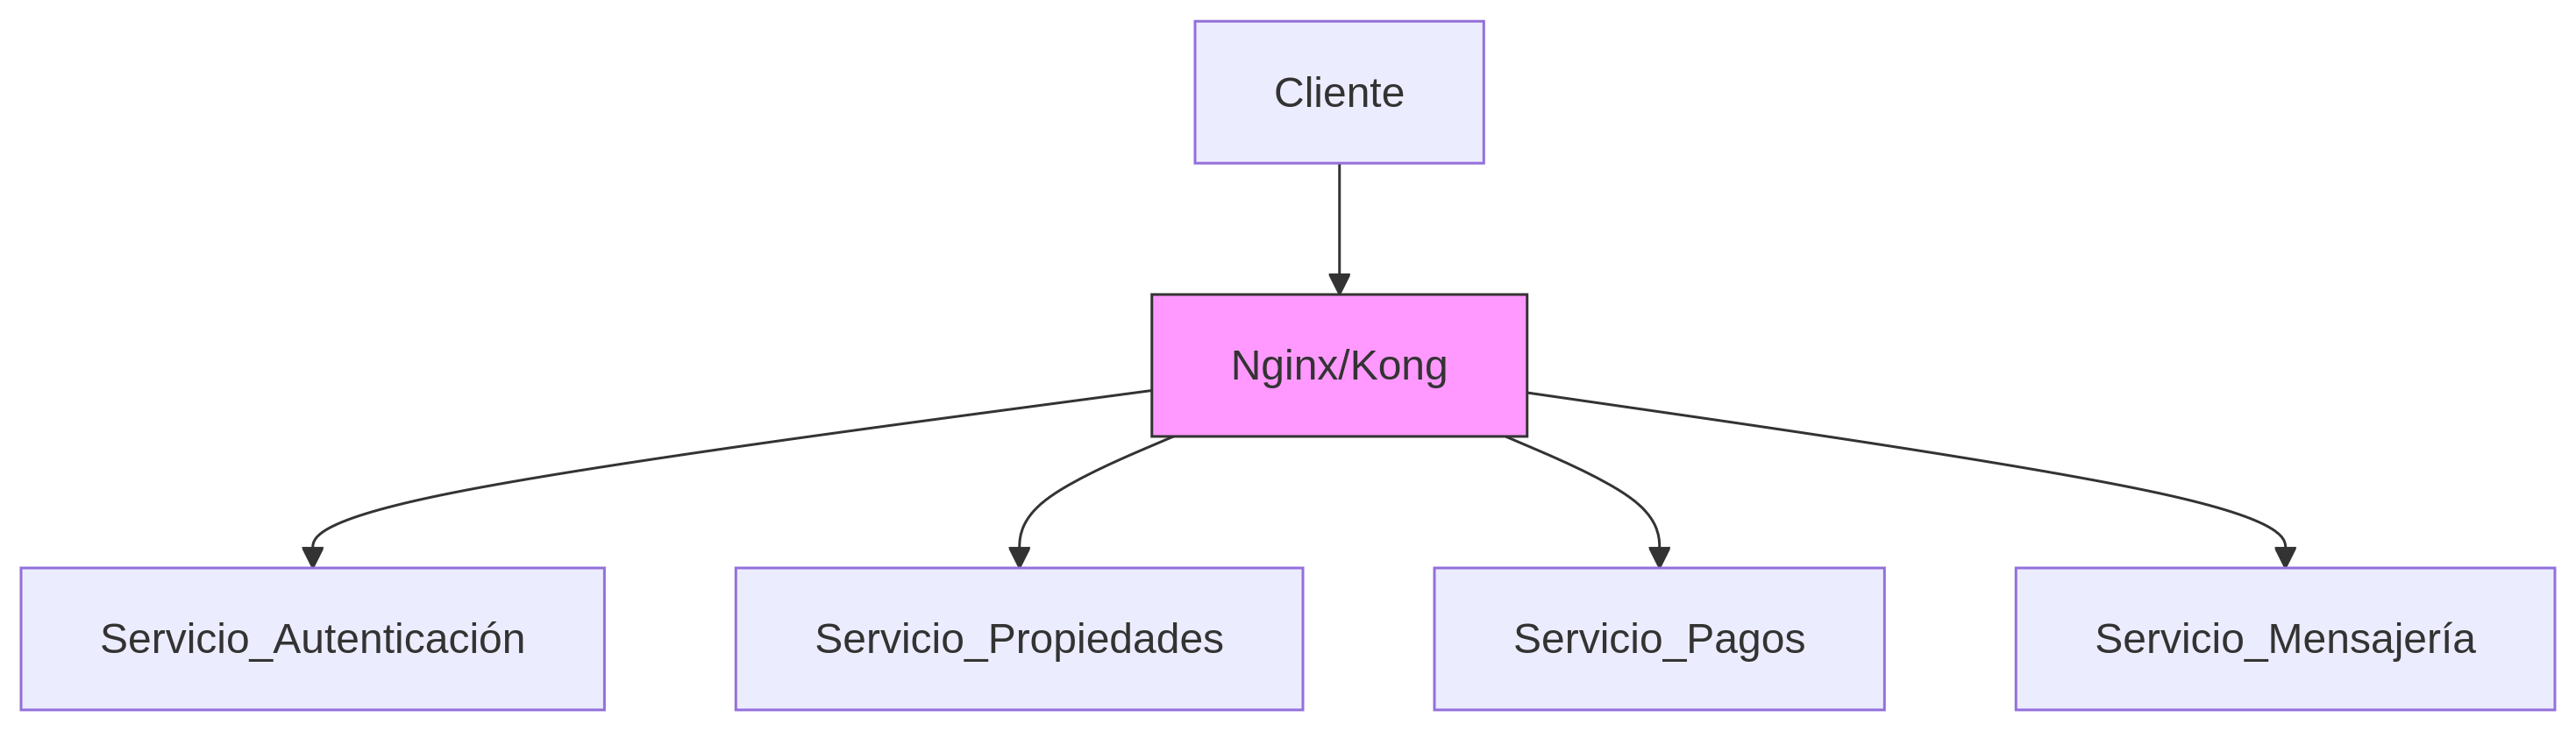
\includegraphics[width=\linewidth]{figures/patterns/APIG.png}
			\captionof{figure}{Componentes API Gateway.}
			\label{fig:img2}
		\end{center}
	
	\subsection*{2. CQRS (Command Query Responsibility Segregation)}
		\begin{itemize}
			\item \textbf{Descripción:} Separa las operaciones de lectura (consultas) de las de escritura (comandos), permitiendo optimizar y escalar cada una por separado.  
			\item \textbf{Aplicación en Casa Fácil:} En funcionalidades como gestión de reservas o propiedades, el modelo de lectura puede ser distinto y más optimizado que el modelo de escritura, por ejemplo, consultas masivas de propiedades vs. edición de una publicación.  
			\item \textbf{Ventajas:}
			\begin{itemize}
				\item Mejora el rendimiento y escalabilidad.
				\item Facilita el uso de diferentes tecnologías para leer y escribir.
				\item Ideal para sistemas con alto volumen de datos y lógica compleja.
			\end{itemize}
		\end{itemize}
		\begin{center}
			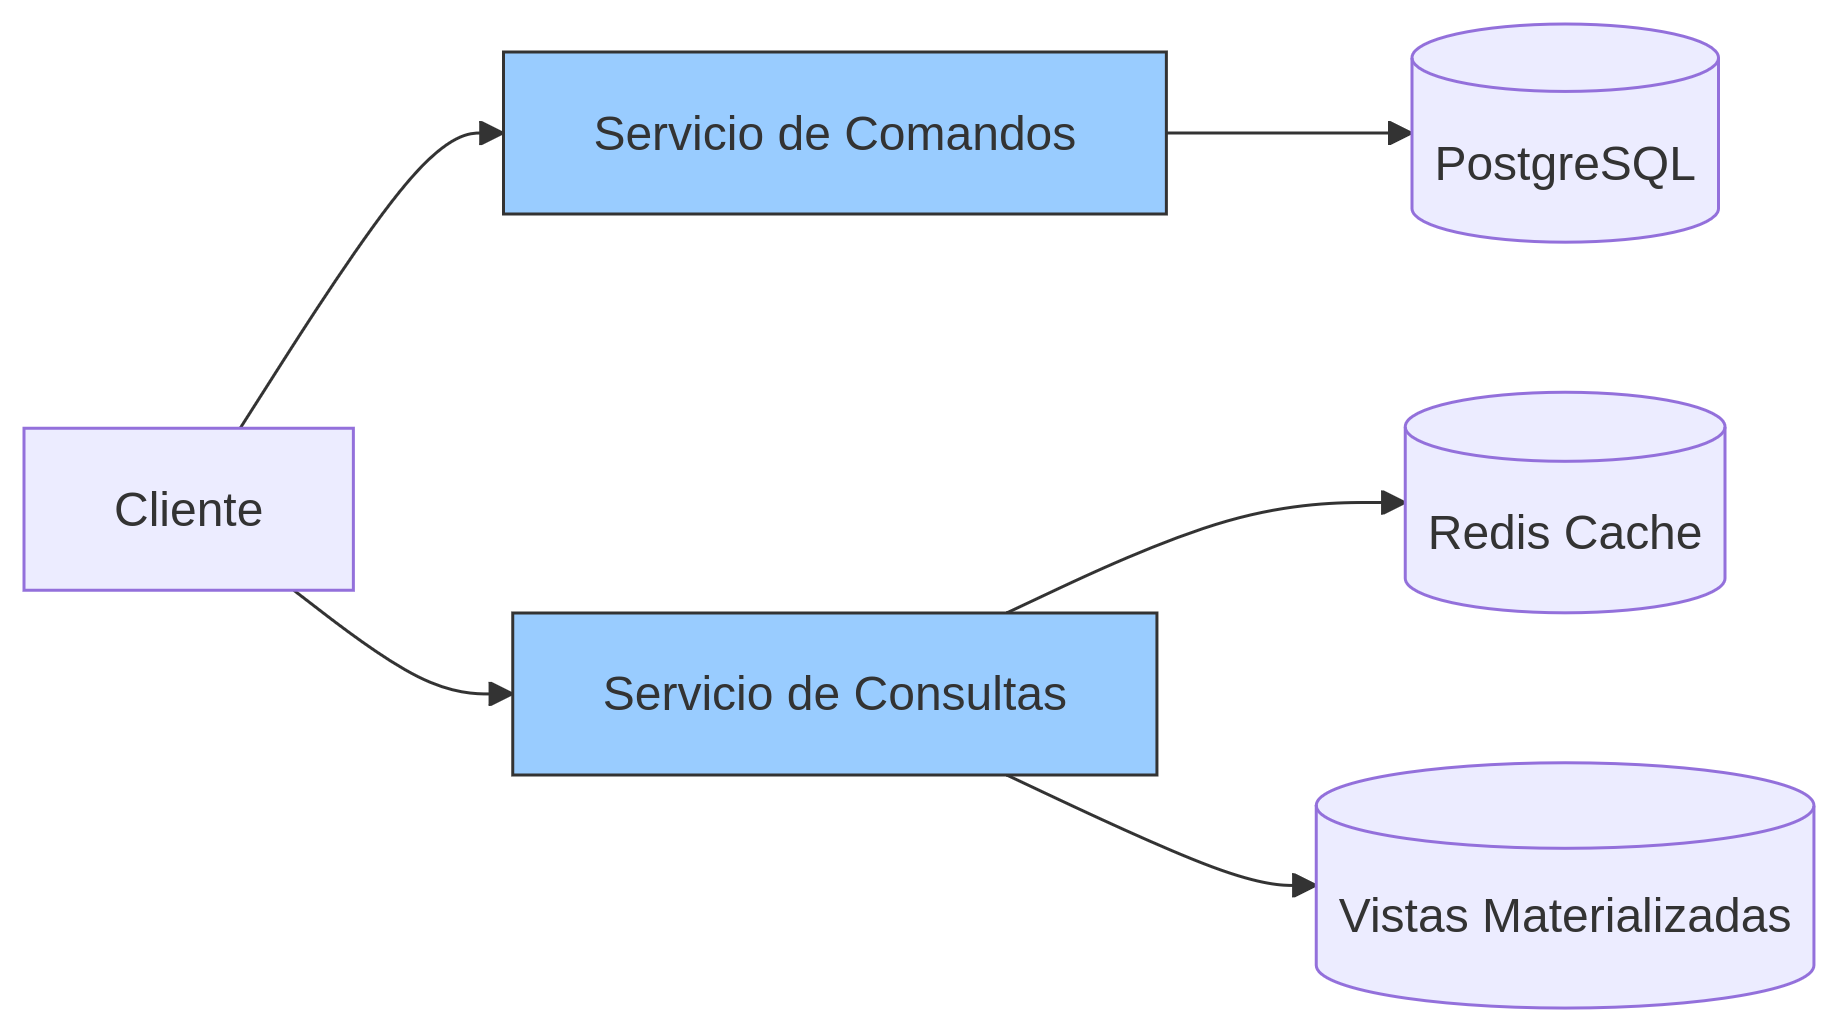
\includegraphics[width=\linewidth]{figures/patterns/CQRS.png}
			\captionof{figure}{Componentes CQRS.}
			\label{fig:img3}
		\end{center}
	
	\subsection*{3. Event Sourcing}
		\begin{itemize}
			\item \textbf{Descripción:} En lugar de almacenar el estado actual de una entidad, se almacena una secuencia de eventos que modificaron su estado.  
			\item \textbf{Aplicación en Casa Fácil:} Para gestionar el historial de reservas, cambios de disponibilidad o pagos, se puede almacenar cada evento como "propiedad reservada", "pago confirmado".  
			\item 	\textbf{Ventajas:}
			\begin{itemize}
				\item Trazabilidad completa de acciones pasadas.
				\item Reversión de cambios y auditoría sencilla.
				\item Se complementa naturalmente con EDA.
			\end{itemize}
		\end{itemize}
		\begin{center}
			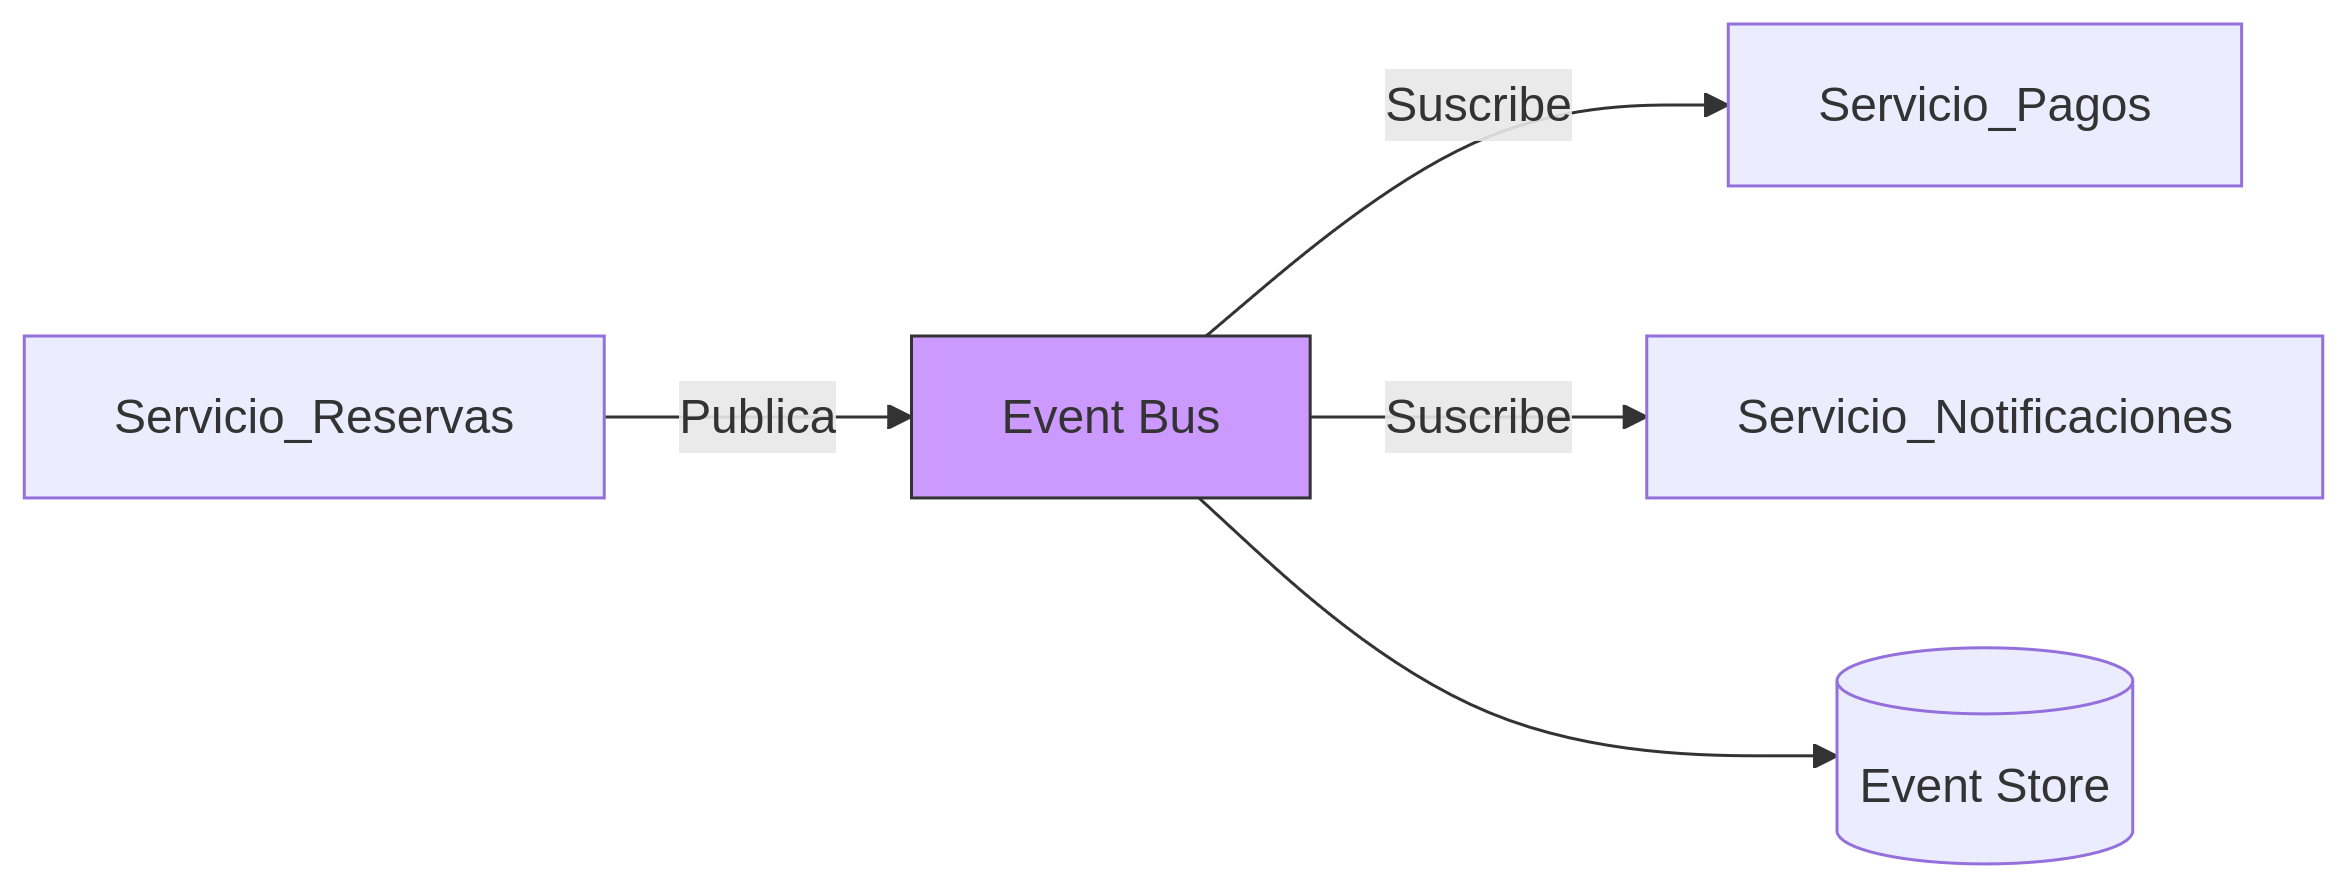
\includegraphics[width=\linewidth]{figures/patterns/EVENT.png}
			\captionof{figure}{Componentes Event Sourcing.}
			\label{fig:img4}
		\end{center}
		
	\subsection*{4. Service Registry \& Discovery}
		\begin{itemize}
			\item \textbf{Descripción:} Permite que los microservicios se registren en un directorio común para ser descubiertos dinámicamente.  
			\item \textbf{Aplicación en Casa Fácil:} En entornos con múltiples servicios desplegados dinámicamente (como en contenedores Docker), el registro facilita la comunicación entre servicios sin direcciones IP fijas.  
			\item 	\textbf{Ventajas:}
			\begin{itemize}
				\item Reducción de la configuración manual.
				\item Mejor soporte para escalado automático.
				\item Necesario para balanceo de carga dinámico.
			\end{itemize}
		\end{itemize}
		\begin{center}
			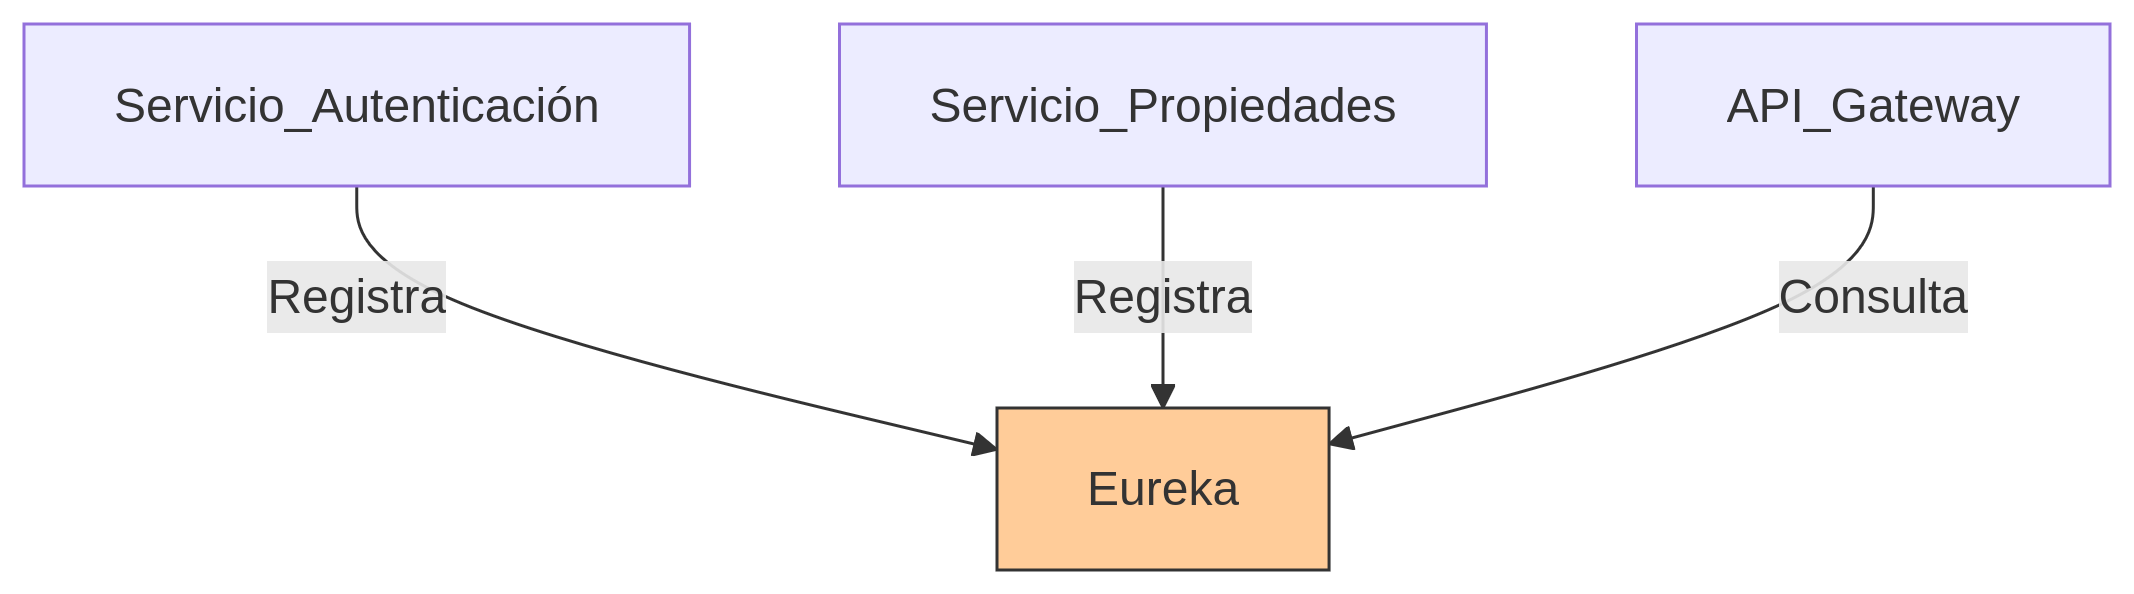
\includegraphics[width=\linewidth]{figures/patterns/SERVICE_R_D.png}
			\captionof{figure}{Componentes Service Registry \& Discovery.}
			\label{fig:img5}
		\end{center}
	
	\subsection*{5. Backend for Frontend (BFF)}
		\begin{itemize}
			\item \textbf{Descripción:} Crea una capa intermedia específica para cada tipo de cliente (web, móvil, etc.), adaptando las respuestas del backend a sus necesidades.  
			\item \textbf{Aplicación en Casa Fácil:} La versión móvil puede tener un BFF que priorice velocidad y respuesta ligera, mientras que la web puede entregar más datos.  
			\item 	\textbf{Ventajas:}
			\begin{itemize}
				\item Reduce carga y complejidad en el frontend.
				\item Mejora la experiencia de usuario según el dispositivo.
				\item Facilita la evolución independiente de interfaces.
			\end{itemize}
		\end{itemize}
		\begin{center}
			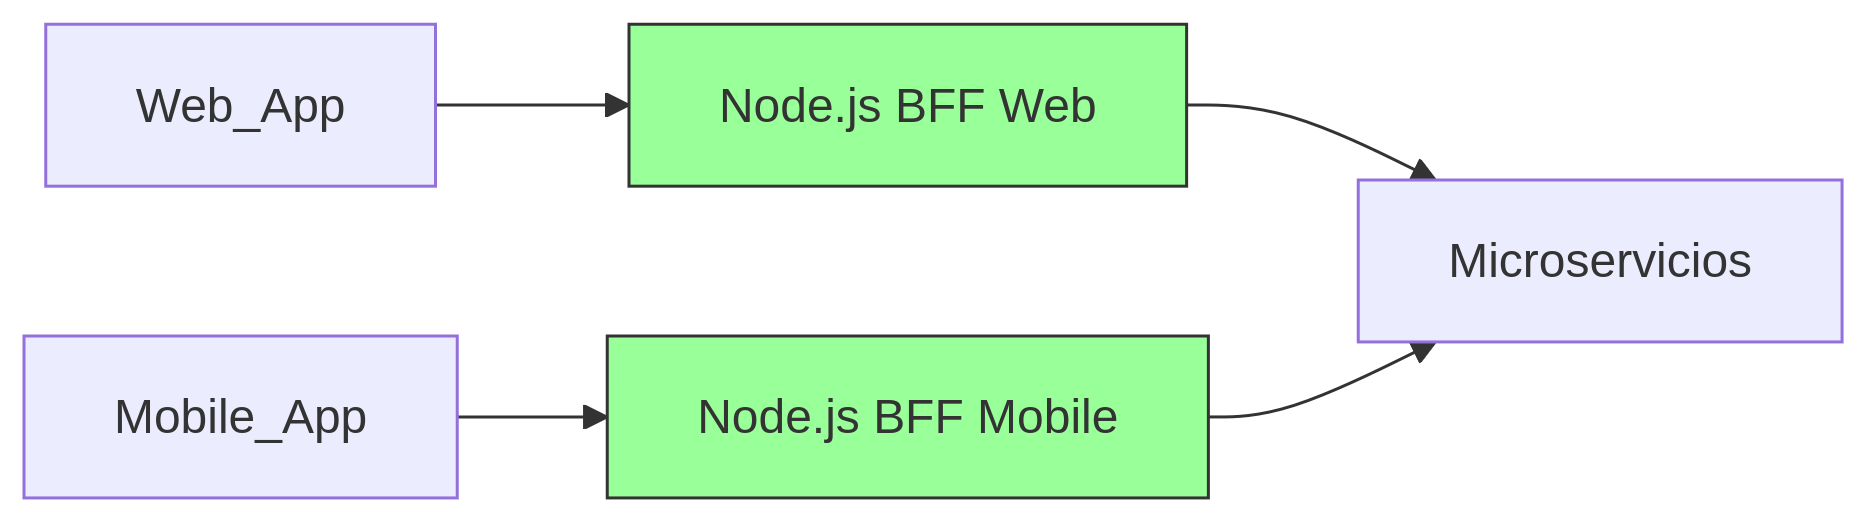
\includegraphics[width=\linewidth]{figures/patterns/BACKEND.png}
			\captionof{figure}{Componentes Backend for Frontend.}
			\label{fig:img6}
		\end{center}
	
	\subsection*{6. Saga}
		\begin{itemize}
			\item \textbf{Descripción:} Coordina transacciones distribuidas entre múltiples servicios, garantizando consistencia eventual a través de una serie de pasos y compensaciones si algo falla.  
			\item \textbf{Aplicación en Casa Fácil:} Una reserva de propiedad puede requerir verificar disponibilidad, generar pago y enviar notificación. Si el pago falla, debe deshacerse todo.  
			\item \textbf{Ventajas:}
			\begin{itemize}
				\item Maneja flujos de negocio complejos sin transacciones bloqueantes.
				\item Aumenta la confiabilidad en flujos asincrónicos.
				\item Escalable y desacoplado.
			\end{itemize}
		\end{itemize}
		\begin{center}
			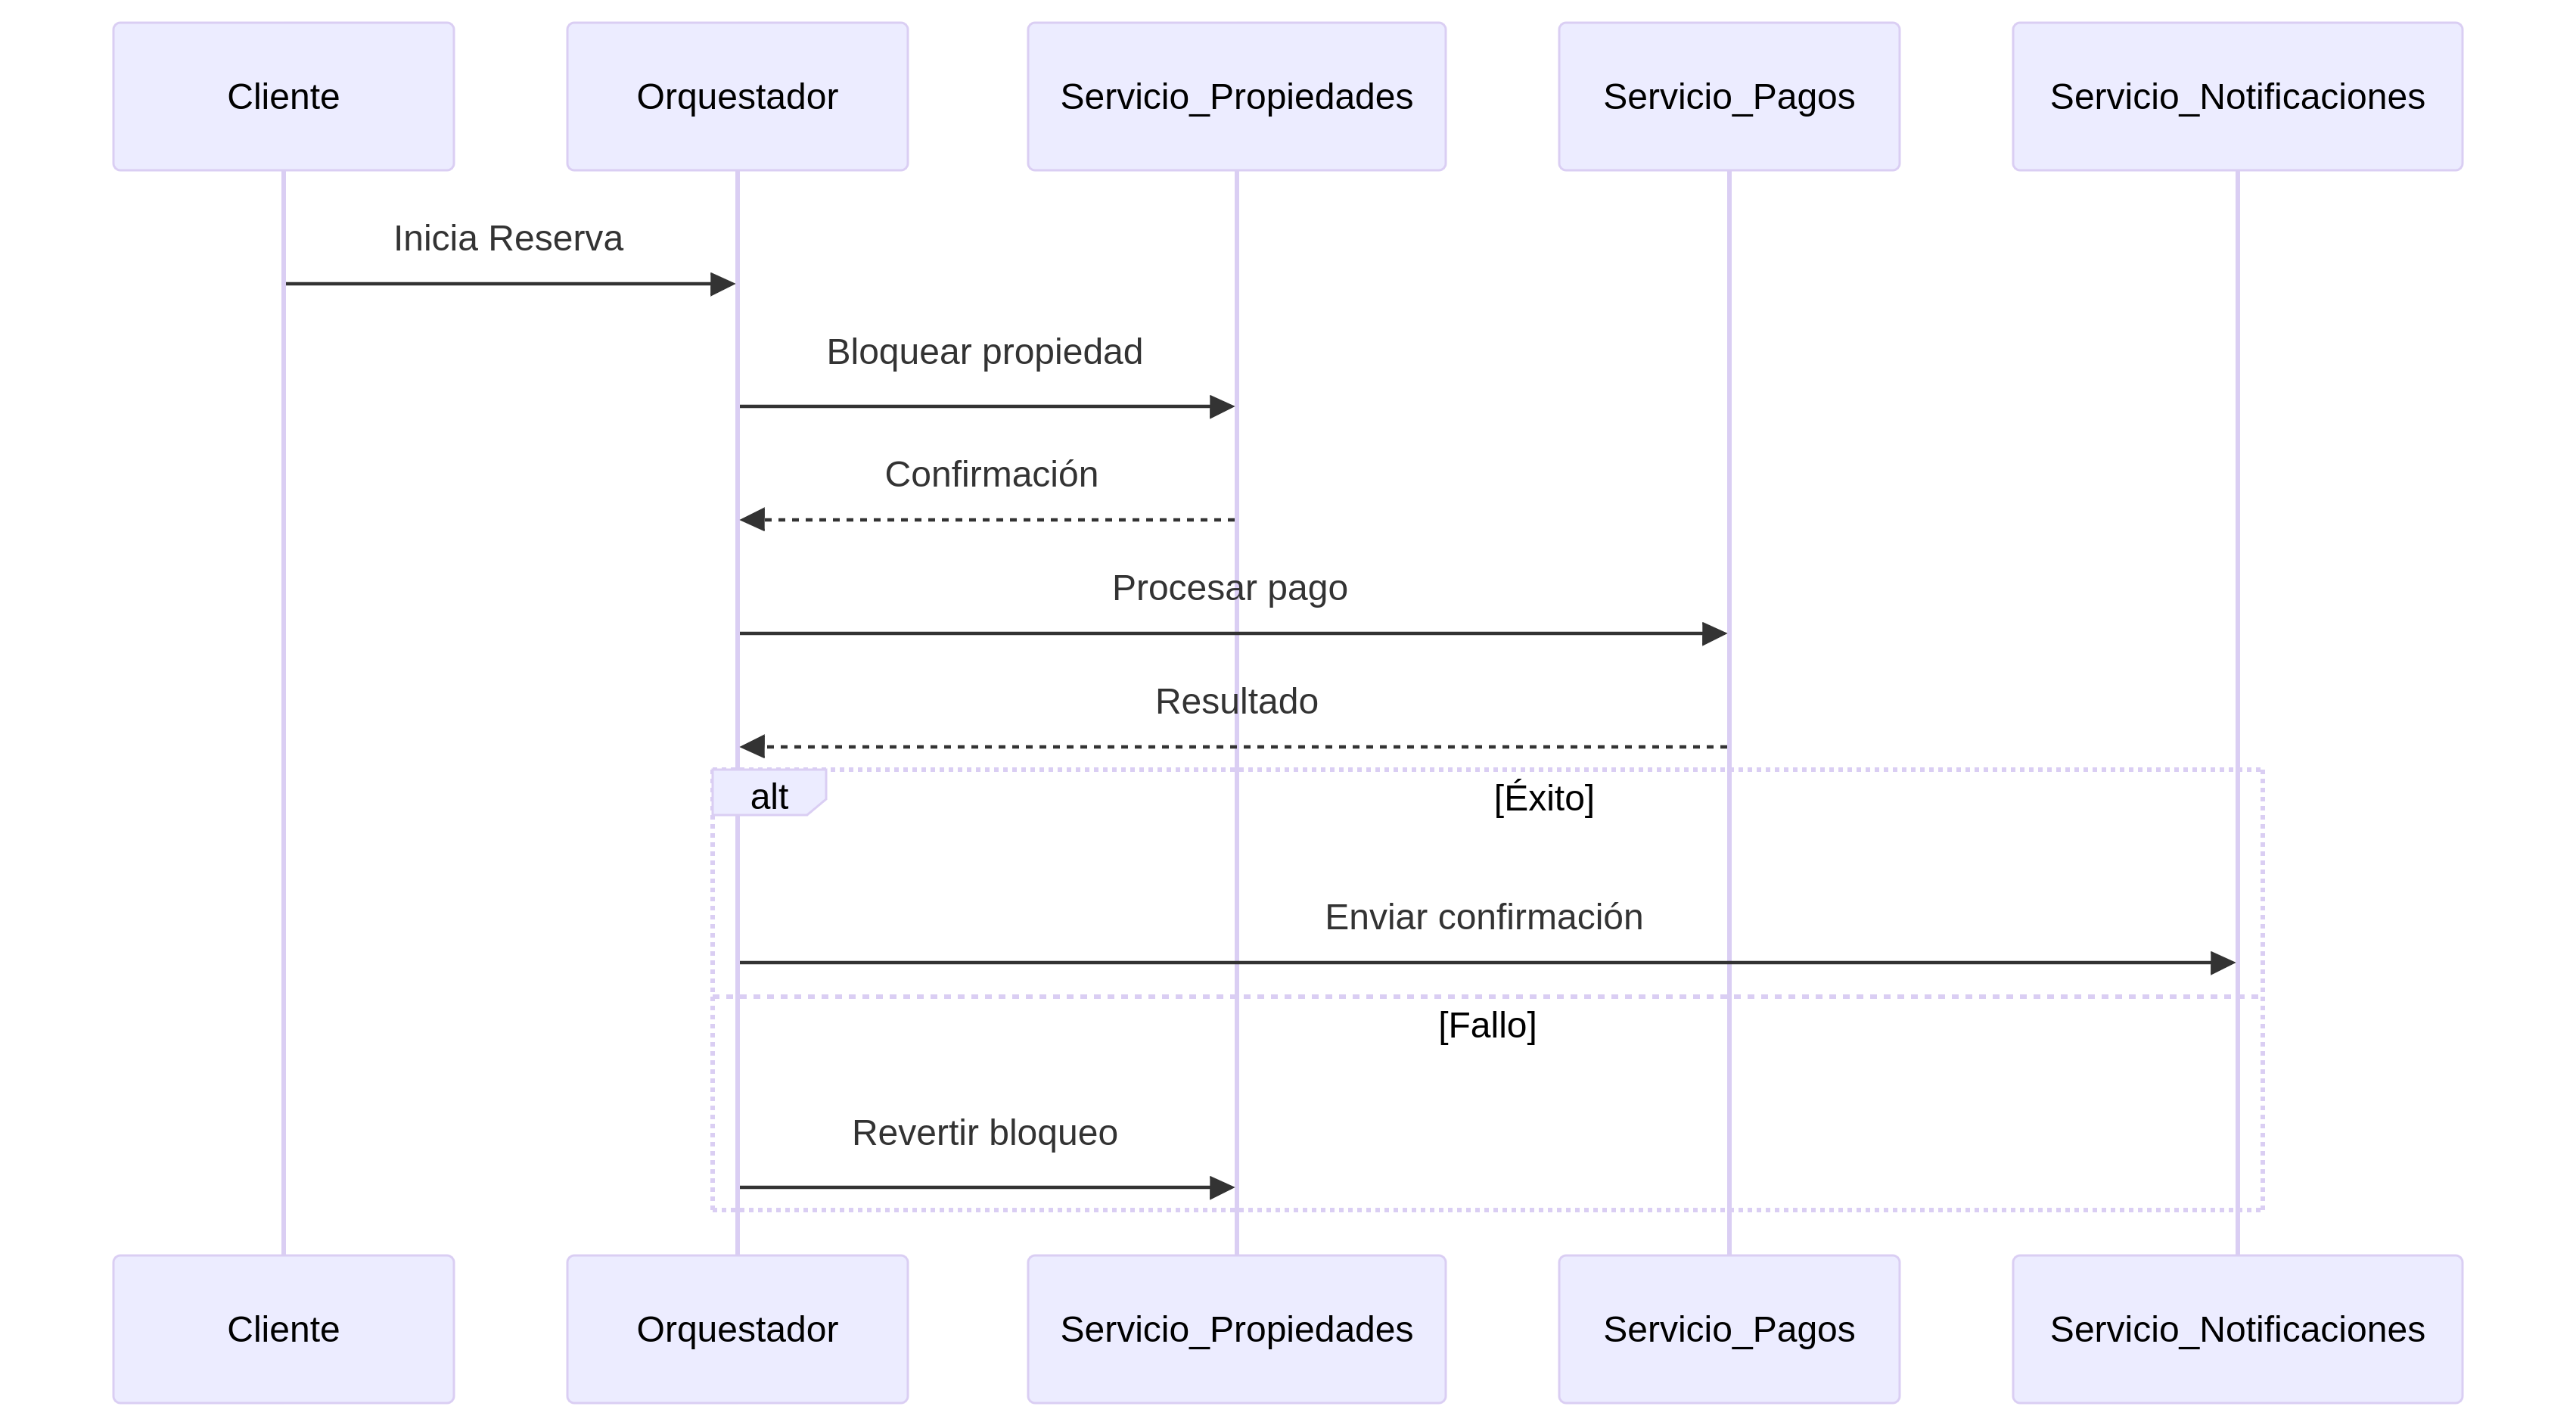
\includegraphics[width=\linewidth]{figures/patterns/SAGA.png}
			\captionof{figure}{Componentes Saga.}
			\label{fig:img7}
		\end{center}
	
	\subsection*{7. Strangler Fig}
		\begin{itemize}
			\item \textbf{Descripción:} Permite reemplazar gradualmente un sistema monolítico por microservicios. Se encapsula el sistema antiguo y se introducen nuevos componentes uno por uno.  
			\item \textbf{Aplicación en Casa Fácil:} Si partes del sistema comienzan siendo monolíticas (como reservas o pagos), pueden migrarse paulatinamente sin interrumpir la operación.  
			\item \textbf{Ventajas:}
			\begin{itemize}
				\item Reducción del riesgo en la migración.
				\item Permite evolución controlada del sistema.
				\item Compatible con despliegue incremental.
			\end{itemize}
		\end{itemize}
		\begin{center}
			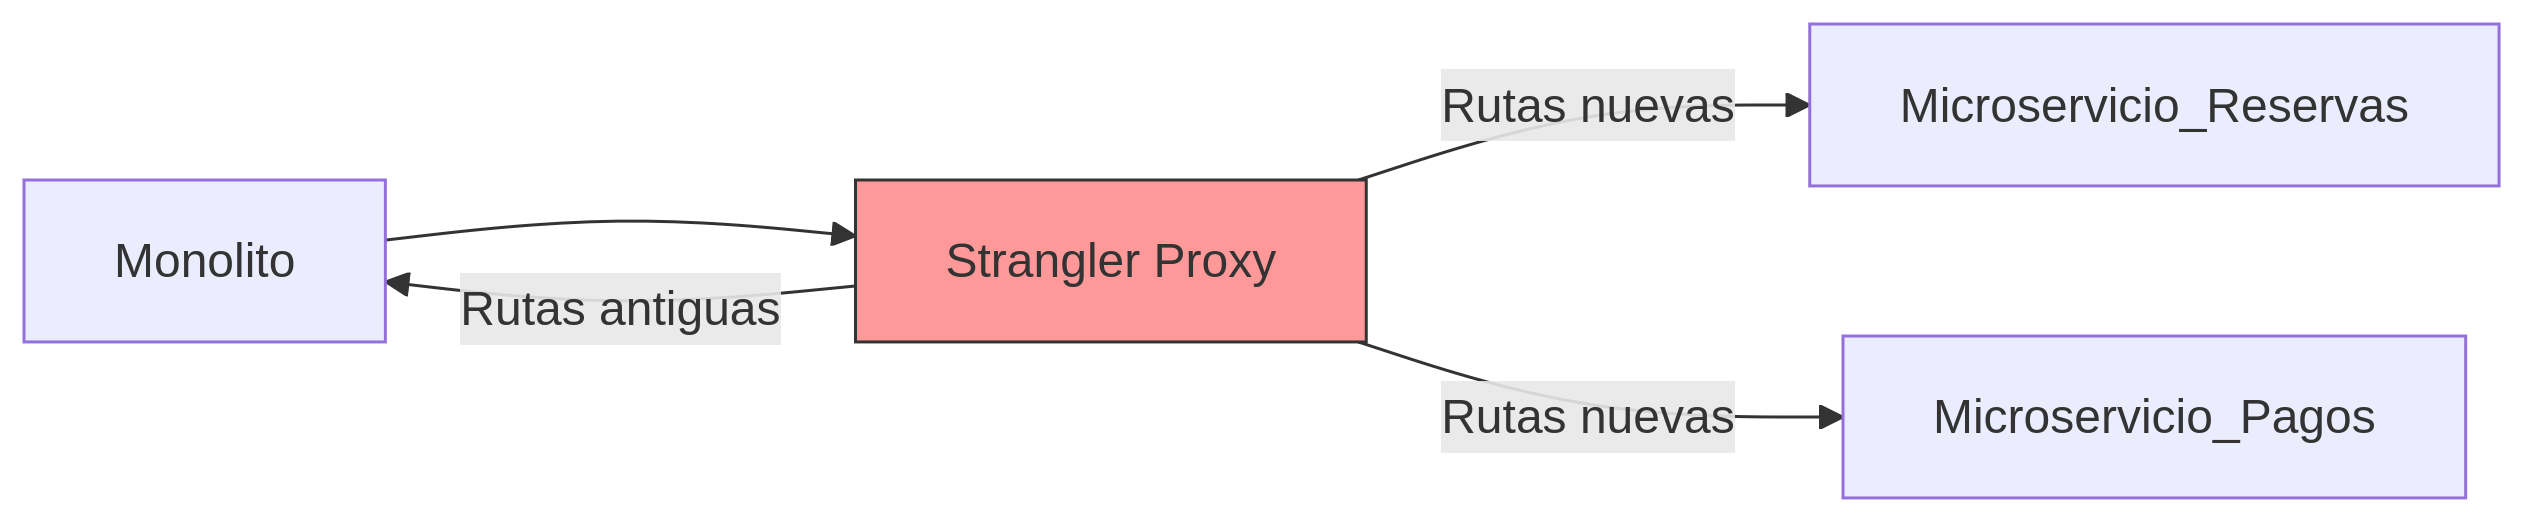
\includegraphics[width=\linewidth]{figures/patterns/STRANGLER.png}
			\captionof{figure}{Componentes Strangler Fig.}
			\label{fig:img8}
		\end{center} \newpage
	\section{Patrones de Diseño}
	\noindent Los patrones de diseño permiten organizar el código de forma flexible, reutilizable y mantenible. A continuación se describen los patrones más relevantes que se aplicarán al sistema \textbf{Casa Fácil}:
	
	\subsection*{1. Strategy Pattern}
		\noindent Este patrón permite definir diferentes algoritmos para una misma tarea y cambiarlos dinámicamente según la necesidad, manteniendo la misma interfaz.  
		\textbf{Aplicación:} En la búsqueda de inmuebles, se pueden aplicar múltiples estrategias: por precio, por cercanía a una universidad o por reglas del inmueble (como "no fumar", "sin mascotas"), sin modificar la lógica principal del buscador.
		\begin{center}
			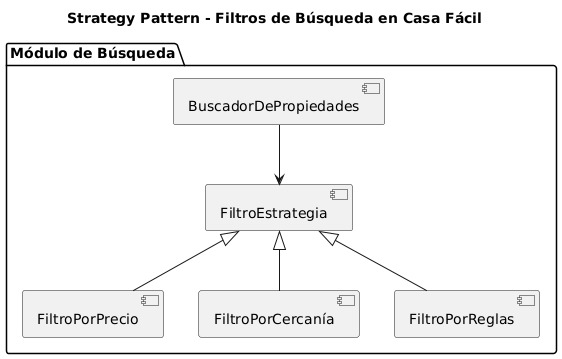
\includegraphics[width=\linewidth]{figures/patterns/strategy.jpg}
			\captionof{figure}{Patron de diseño Strategy.}
			\label{fig:img9}
		\end{center}
	
	\subsection*{2. Observer Pattern}
		\noindent Define una relación de dependencia uno-a-muchos, de modo que cuando un objeto cambia de estado, todos los observadores reciben notificaciones automáticamente.  
		\textbf{Aplicación:} Los usuarios que se suscriban a una propiedad recibirán notificaciones automáticas cuando cambie su disponibilidad o precio.
		\begin{center}
			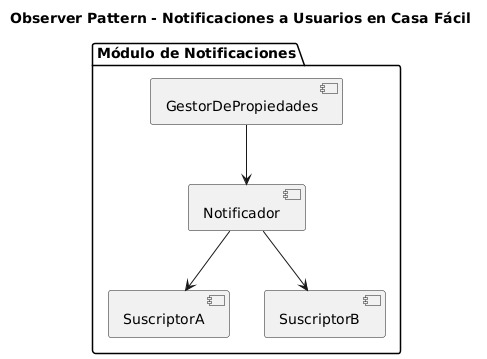
\includegraphics[width=\linewidth]{figures/patterns/observe.jpg}
			\captionof{figure}{Patrón de diseño Observer.}
			\label{fig:img10}
		\end{center}
	
	\subsection*{3. Facade Pattern}
		\noindent Proporciona una interfaz unificada y simplificada a un conjunto de funcionalidades complejas.  
		\textbf{Aplicación:} Puede encapsular toda la lógica de reservas, pagos o validaciones en una clase fachada, de modo que el frontend interactúe con un solo punto de entrada, simplificando las integraciones.
		\begin{center}
			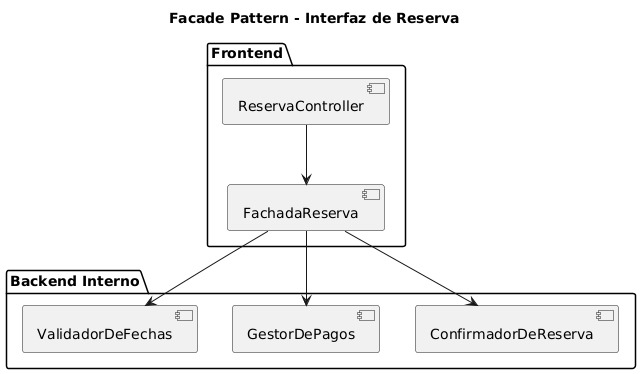
\includegraphics[width=\linewidth]{figures/patterns/facade.jpg}
			\captionof{figure}{Patrón de diseño Facade.}
			\label{fig:img11}
		\end{center}
	
	\subsection*{4. Decorator Pattern}
		\noindent Permite extender dinámicamente el comportamiento de un objeto envolviéndolo con nuevos componentes, sin modificar su clase original.  
		\textbf{Aplicación:} El sistema de notificaciones puede comenzar con envíos por correo electrónico, y luego extenderse fácilmente a SMS o WhatsApp mediante decoradores.
		\begin{center}
			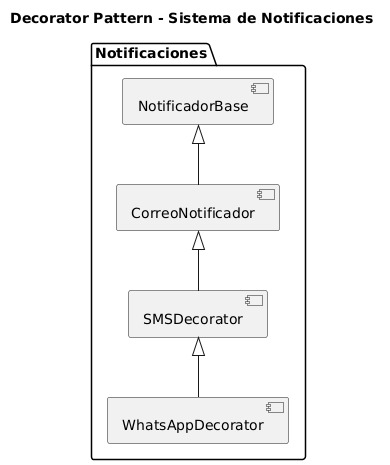
\includegraphics[width=\linewidth]{figures/patterns/decorator.jpg}
			\captionof{figure}{Patrón de diseño Decorator.}
			\label{fig:img12}
		\end{center}
	
	\subsection*{5. Singleton Pattern}
		\noindent Garantiza que una clase tenga una única instancia durante todo el ciclo de vida del sistema, y proporciona un acceso global a ella.  
		\textbf{Aplicación:} Puede utilizarse para gestionar una única instancia del sistema de configuración o autenticación del sistema.
		\begin{center}
			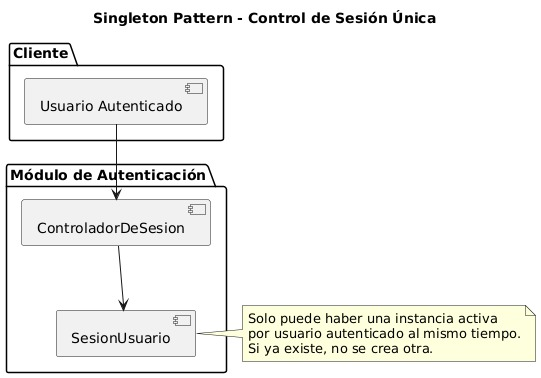
\includegraphics[width=\linewidth]{figures/patterns/singleton.jpg}
			\captionof{figure}{Patrón de diseño Singleton.}
			\label{fig:img13}
		\end{center}
	
	\subsection*{6. Factory Pattern}
		\noindent Permite crear objetos sin exponer su lógica de creación al cliente, utilizando una interfaz común.  
		\textbf{Aplicación:} Se puede usar para crear diferentes tipos de usuarios (inquilino, propietario, administrador), propiedades o métodos de pago, desde una misma factoría base.
		\begin{center}
			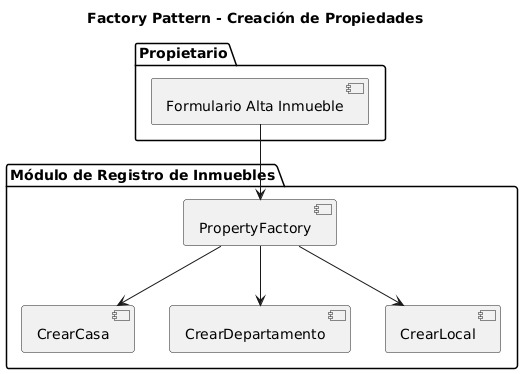
\includegraphics[width=\linewidth]{figures/patterns/factory.jpg}
			\captionof{figure}{Patrón de diseño Factory.}
			\label{fig:img14}
		\end{center}
	
	\subsection*{7. Repository Pattern}
		\noindent Actúa como una capa intermedia entre la lógica de negocio y la base de datos, permitiendo un acceso estructurado y mantenible.  
		\textbf{Aplicación:} Se puede aplicar para generar repositorios reutilizables de entidades como propiedades, usuarios o mensajes.
		\begin{center}
			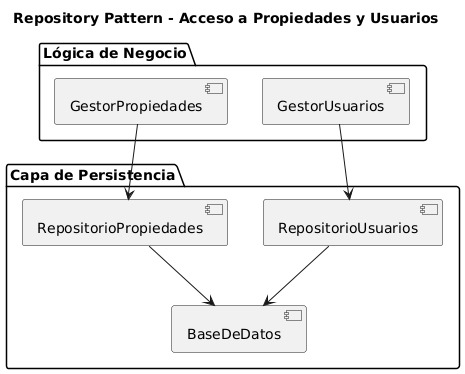
\includegraphics[width=\linewidth]{figures/patterns/repository.jpg}
			\captionof{figure}{Patrón de diseño Repository.}
			\label{fig:img15}
		\end{center}
	
	\subsection*{8. Composite Pattern}
		\noindent Permite tratar objetos individuales y estructuras jerárquicas de manera uniforme.  
		\textbf{Aplicación:} Es útil para representar jerarquías de reglas (por ejemplo, reglas generales y subreglas por inmueble), o categorías y subcategorías de propiedades (como “Habitaciones” → “Amuebladas” / “Sin amueblar”).
		\begin{center}
			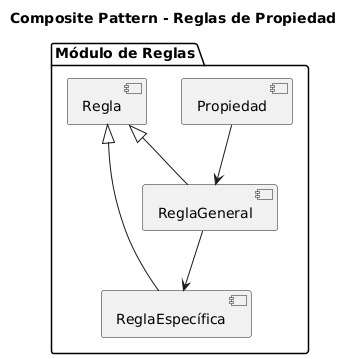
\includegraphics[width=\linewidth]{figures/patterns/composite.jpg}
			\captionof{figure}{Patrón de diseño Composite.}
			\label{fig:img16}
		\end{center}
		
	\subsection*{9. Lazy Loading}
		\noindent Retrasa la carga de recursos hasta que realmente se necesitan.  
		\textbf{Aplicación:} Imágenes, videos, mapas o reseñas de propiedades pueden cargarse solo cuando el usuario interactúe con ellos, mejorando así el rendimiento general del sistema.
		\begin{center}
			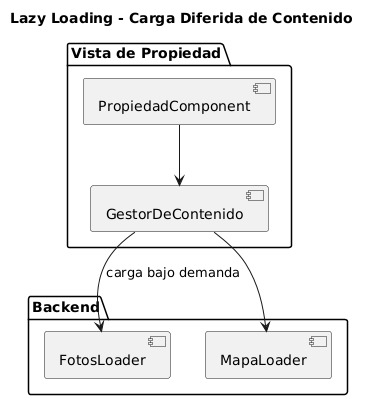
\includegraphics[width=\linewidth]{figures/patterns/lazy.jpg}
			\captionof{figure}{Patrón de diseño Lazy Loading.}
			\label{fig:img17}
		\end{center}
		
	\newpage
	\subsection*{10. Principios SOLID}
		\noindent Los principios SOLID permiten crear software más mantenible, modular y fácil de probar. Son esenciales al trabajar con microservicios y arquitecturas escalables como la de \textbf{Casa Fácil}.
		
		\begin{itemize}
			\item \textbf{S - Single Responsibility Principle:} Cada clase debe tener una única responsabilidad. En Casa Fácil, por ejemplo, un servicio dedicado solo a manejar pagos o reservas.
			
			\item \textbf{O - Open/Closed Principle:} El código debe estar abierto a extensión, pero cerrado a modificación. Por ejemplo, al agregar nuevas formas de pago sin alterar el código original, se puede usar el patrón Strategy.
			
			\item \textbf{L - Liskov Substitution Principle:} Las clases derivadas deben poder sustituir a sus clases base sin afectar el funcionamiento. Por ejemplo, una clase \texttt{UsuarioPremium} debe poder sustituir a \texttt{Usuario} sin romper la lógica.
			
			\item \textbf{I - Interface Segregation Principle:} Es mejor tener interfaces pequeñas y específicas que una general demasiado extensa. Un controlador de publicaciones no debería forzarse a implementar métodos de notificación si no los necesita.
			
			\item \textbf{D - Dependency Inversion Principle:} Las clases deben depender de abstracciones, no de clases concretas. Esto permite inyectar servicios como repositorios o validadores sin acoplarlos al código del controlador.
		\end{itemize} \newpage
	\section{Diagramas}
	\subsection{Diagrama de componenes.}
	\begin{center}
		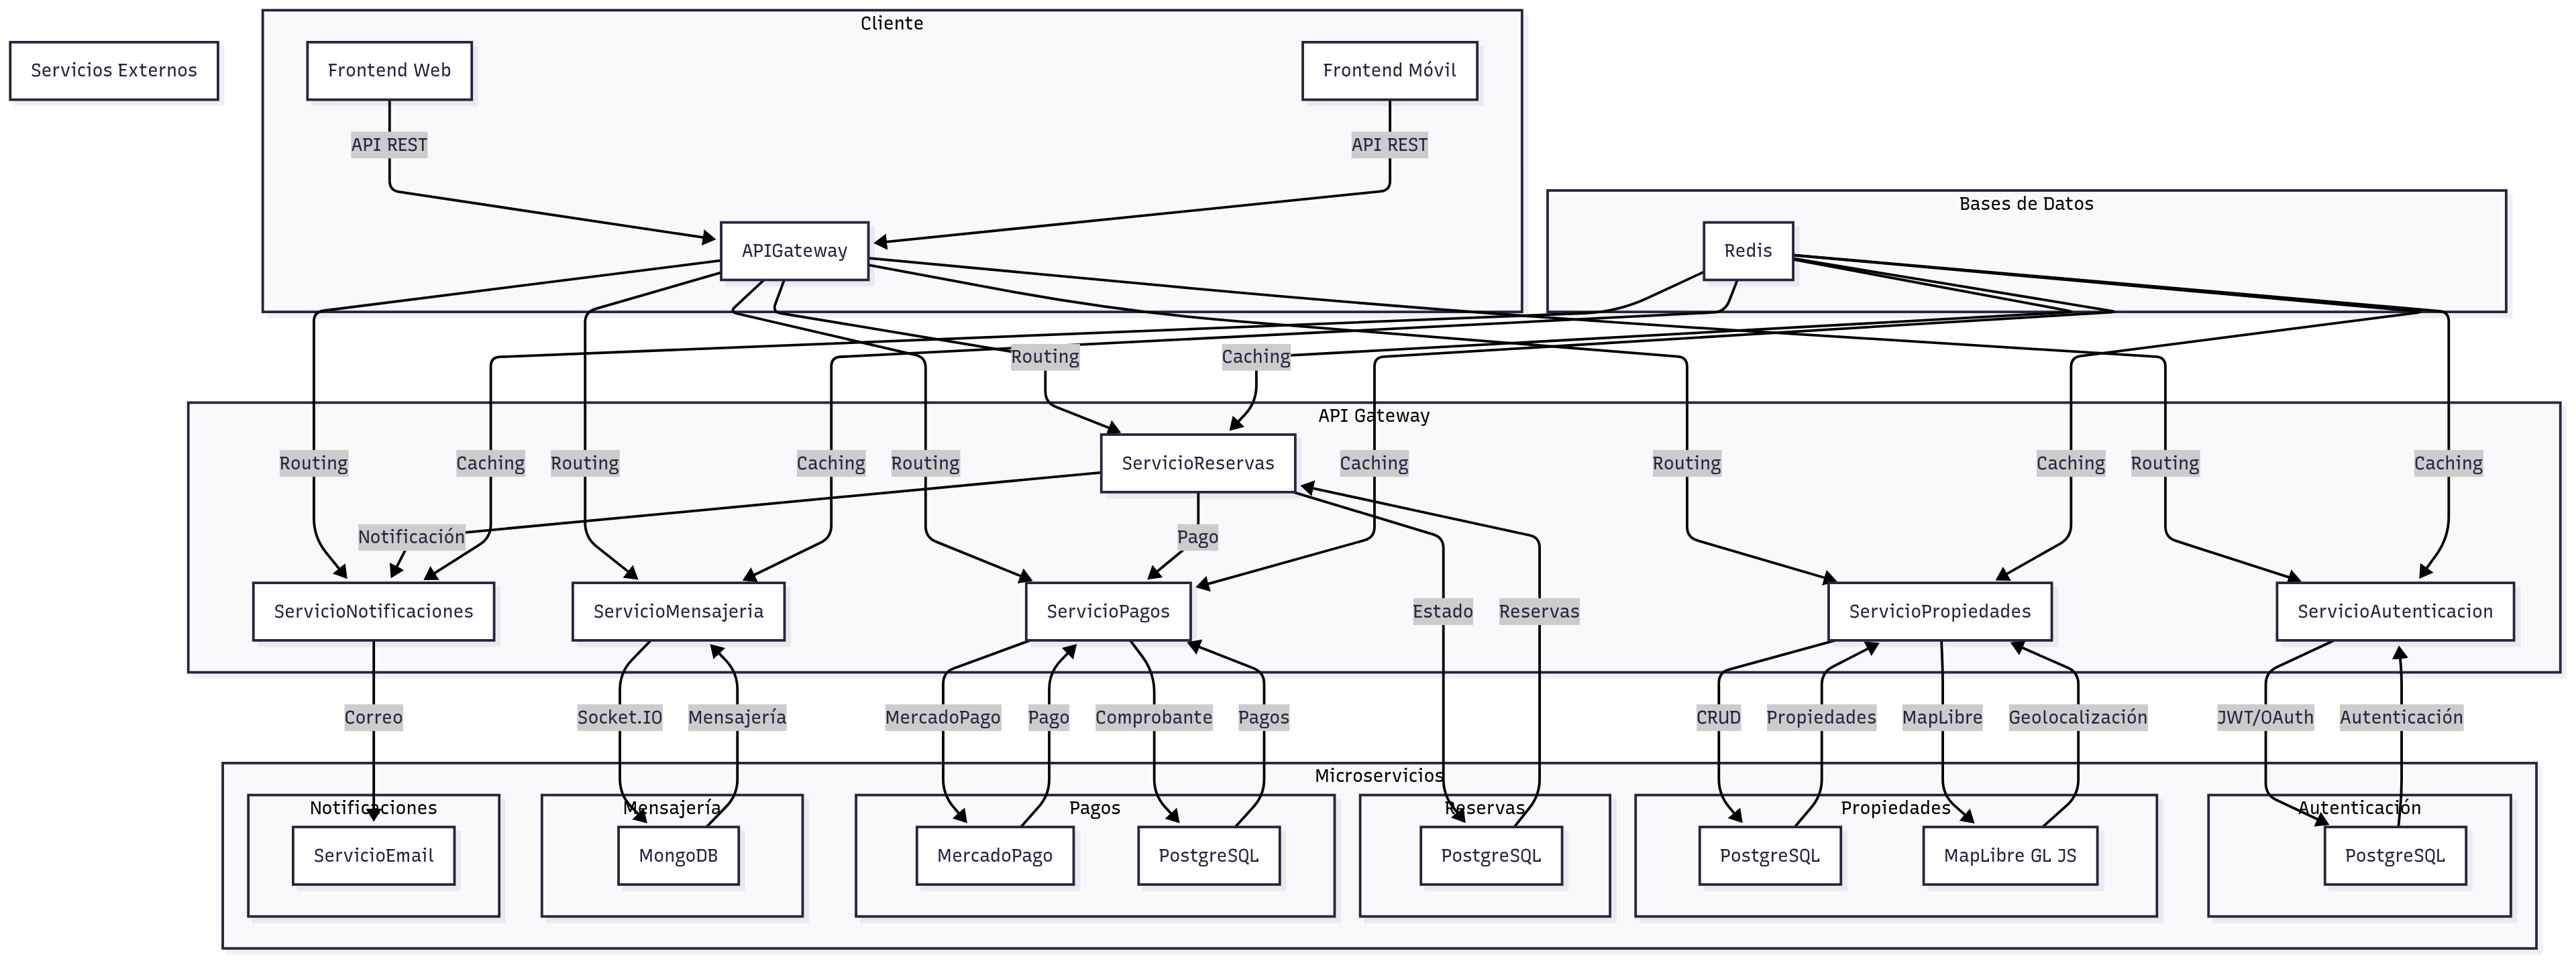
\includegraphics[width=\linewidth]{figures/diagrams/Diagrama conceptual del sistema.png}
		\captionof{figure}{Diagrama de Componntes.}
		\label{fig:img90}
	\end{center}
	\subsection{Diagrama de patrones y estilo.}
	\begin{center}
		\includegraphics[width=\linewidth]{figures/diagrams/Diagrama de patrones y estilo arquitectónico.png}
		\captionof{figure}{Diagrama de Patrones y Estilo Arquitectónico.}
		\label{fig:img100}
	\end{center}
	\subsection{Diagrama de Clases Inicial con Entidades Principales y Relaciones.}
	\begin{center}
		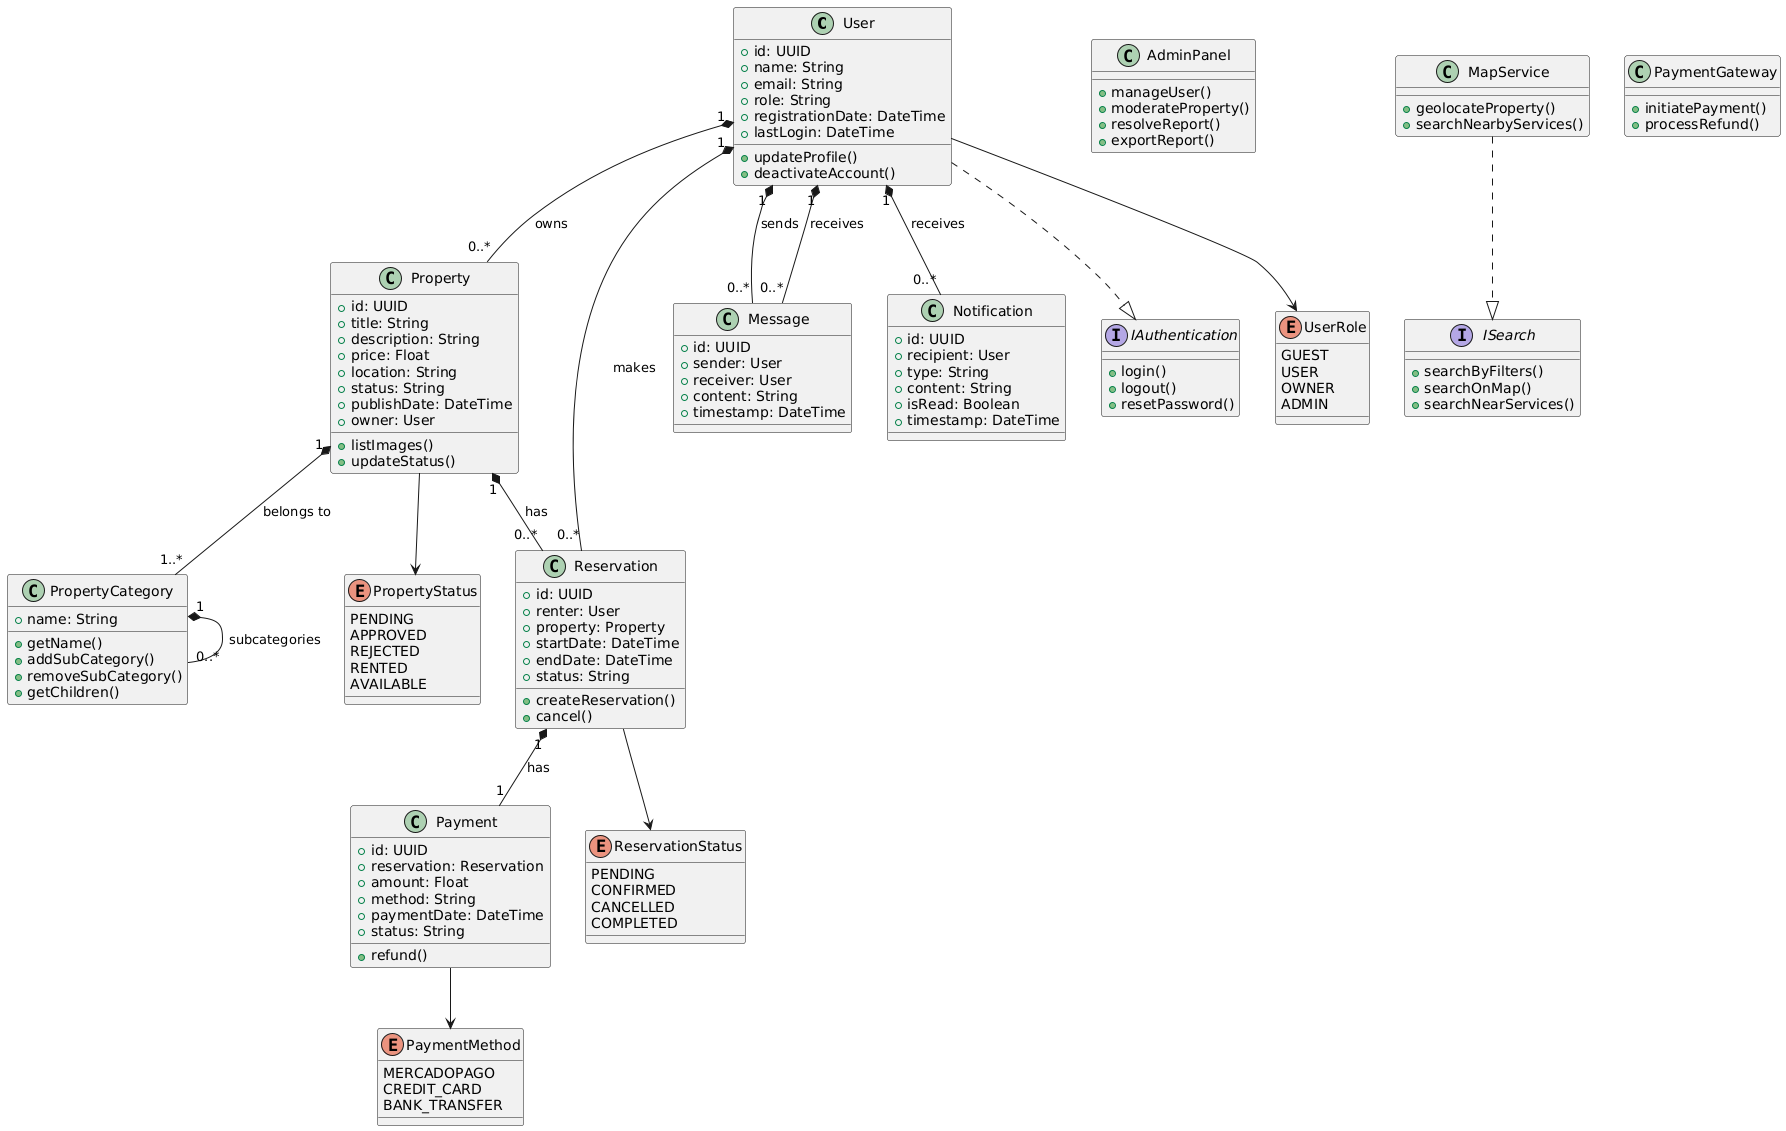
\includegraphics[width=\linewidth]{figures/diagrams/Diagrama de Clases.png}
		\captionof{figure}{Diagrama de Clases.}
		\label{fig:img110}
	\end{center} \newpage
	\section{Resumen del Sistema}
	\noindent El sistema \textit{Casa Fácil} incluye una serie de funcionalidades esenciales que permiten a los usuarios interactuar eficientemente entre sí y con el sistema. A continuación, se detallan todas las funcionalidades clave:
	
	\subsection*{Autenticación y Gestión de Usuarios}
		\begin{itemize}
			\item \textbf{Registro de usuarios}: Permite a nuevos usuarios registrarse mediante un formulario en línea o mediante OAuth.
			\item \textbf{Inicio de sesión}: Los usuarios pueden iniciar sesión con sus credenciales.
			\item \textbf{Recuperación de contraseña}: Los usuarios pueden recuperar el acceso a su cuenta mediante un enlace enviado a su correo electrónico.
			\item \textbf{Gestión de roles y permisos}: El sistema permite diferenciar funcionalidades según el rol (usuario autenticado, usuario no autenticado, propietario o administrador).
			\item \textbf{Verificación de identidad del propietario}: El sistema debe verificar la identidad del propietario como dueño o administrador del inmueble.
			\item \textbf{Cierre de sesión seguro}: El sistema permite a los usuarios cerrar su sesión de forma segura.
			\item \textbf{Gestión de perfil}: Los usuarios pueden actualizar su información personal, foto y preferencias desde su perfil.
			\item \textbf{Eliminación o desactivación de cuenta}: Los usuarios pueden eliminar o desactivar su cuenta conforme a la política de privacidad.
		\end{itemize}
	
	\subsection*{Gestión de Propiedades}
		\begin{itemize}
			\item \textbf{Visualización de propiedades}: Los usuarios pueden ver las propiedades disponibles en la plataforma con información básica.
			\item \textbf{Detalles de propiedad}: Al seleccionar una propiedad, se muestran su información adicional, incluyendo galería, descripción, precio, ubicación, subcategorías y reseñas.
			\item \textbf{Creación de propiedades}: Los usuarios con rol propietario pueden registrar nuevas propiedades para rentar.
			\item \textbf{Edición y eliminación de propiedades}: Los propietarios o administradores pueden modificar o eliminar propiedades previamente publicadas.
			\item \textbf{Publicación programada de propiedades}: Los propietarios pueden seleccionar una fecha futura para la publicación automática de sus propiedades.
			\item \textbf{Revisión/moderación de propiedades por administrador}: Las propiedades registradas son revisadas por un administrador antes de ser visibles en la plataforma.
		\end{itemize}
	
	\subsection*{Búsqueda y Exploración}
		\begin{itemize}
			\item \textbf{Búsqueda de propiedades}: El sistema permite a los usuarios buscar propiedades mediante filtros avanzados (precio, tipo, ubicación, categoría).
			\item \textbf{Búsqueda en mapa interactivo}: Los resultados de búsqueda se visualizan geográficamente sobre un mapa interactivo.
			\item \textbf{Búsqueda por cercanía a servicios clave}: El sistema permite filtrar propiedades según su proximidad a lugares de interés (universidades, transporte, hospitales, etc.).
		\end{itemize}
	
	\subsection*{Interacción del Usuario}
		\begin{itemize}
			\item \textbf{Favoritos}: Los usuarios pueden marcar propiedades como favoritas para acceder fácilmente a ellas.
			\item \textbf{Solicitud de reserva}: Los usuarios autenticados pueden enviar una solicitud para reservar una propiedad.
			\item \textbf{Agendamiento de citas}: Los usuarios pueden agendar visitas presenciales o virtuales con los propietarios.
			\item \textbf{Reserva de propiedad}: Los usuarios pueden reservar temporalmente una propiedad mediante pago anticipado.
			\item \textbf{Mensajería interna}: Los usuarios pueden enviar mensajes a los propietarios directamente desde la plataforma.
			\item \textbf{Calificación y reseña}: Los usuarios pueden calificar y dejar reseñas después de completar una transacción.
			\item \textbf{Reporte de usuarios o publicaciones}: Los usuarios pueden reportar publicaciones sospechosas o usuarios con comportamiento inadecuado.
			\item \textbf{Notificaciones internas y por correo}: El sistema envía notificaciones relevantes dentro de la aplicación y por medio de correo electrónico.
		\end{itemize}
	
	\subsection*{Pagos, Transacciones y Facturas}
		\begin{itemize}
			\item \textbf{Opciones de pago}: El sistema permite a los usuarios realizar pagos mediante la pasarela de pago de Mercado Pago.
			\item \textbf{Generación de comprobante}: Tras una transacción exitosa, se genera un comprobante en PDF con los detalles.
			\item \textbf{Historial de rentas}: Los usuarios pueden consultar su historial de rentas.
			\item \textbf{Gestión de reembolsos}: Los usuarios pueden solicitar reembolsos según las políticas establecidas.
		\end{itemize}
	
	\subsection*{Panel de Administración}
		\begin{itemize}
			\item \textbf{Panel de administración}: El sistema permite a los administradores gestionar usuarios, propiedades, reservas y transacciones.
			\item \textbf{Gestión de reportes de usuarios}: Los administradores pueden revisar reportes realizados por los usuarios sobre contenidos o comportamientos inadecuados.
			\item \textbf{Estadísticas por periodo de tiempo}: El sistema permite visualizar métricas clave como usuarios activos, ingresos y publicaciones.
			\item \textbf{Exportación de datos y reportes}: Los administradores pueden exportar reportes en formatos como CSV, PDF, Excel, etc.
		\end{itemize}
	
	\subsection*{Servicios Complementarios}
		\begin{itemize}
			\item \textbf{Integración de servicios locales}: El sistema conecta con APIs de mapas y servicios externos para mostrar información sobre lavanderías, estacionamientos, transporte y otros servicios cercanos a las propiedades.
		\end{itemize}
	
	\subsection*{Seguridad y Control de Acceso}
		\begin{itemize}
			\item \textbf{Control de roles y permisos}: El sistema permite diferenciar funcionalidades según el rol (usuario autenticado, usuario no autenticado, propietario o administrador).
			\item \textbf{Verificación de identidad del propietario}: El sistema debe verificar la identidad del propietario como dueño o administrador del inmueble.
			\item \textbf{Autenticación y autorización}: El sistema gestiona el acceso mediante JWT/OAuth y controla qué funcionalidades puede usar cada usuario según su rol.
		\end{itemize}
	
	\subsection*{Arquitectura y Diseño Técnico}
		\begin{itemize}
			\item \textbf{Microservicios}: El sistema se divide en múltiples servicios pequeños, autónomos y especializados, como el servicio de cuentas, el servicio de pago, el servicio de mapas, y el servicio de mensajería.
			\item \textbf{API Gateway}: Centraliza las solicitudes del cliente y las enruta a los servicios correspondientes.
			\item \textbf{Base de datos}: Almacena datos relacionales (PostgreSQL) y no estructurados (MongoDB), junto con caché y sesiones (Redis).
			\item \textbf{Event Sourcing}: Almacena eventos en lugar de estados actuales, facilitando la trazabilidad y auditoría.
			\item \textbf{Service Registry \& Discovery}: Facilita la comunicación entre microservicios sin necesidad de direcciones IP fijas.
			\item \textbf{Backend for Frontend (BFF)}: Crea capas intermedias específicas para cada tipo de cliente (web, móvil), adaptando las respuestas del backend a sus necesidades.
		\end{itemize}
	
	\subsection*{Diseño y Experiencia de Usuario}
		\begin{itemize}
			\item \textbf{Interfaz intuitiva}: La interfaz debe ser fácil de entender y usar, con flujos de usuario claros y retroalimentación inmediata.
			\item \textbf{Accesibilidad}: El sistema debe cumplir con estándares de accesibilidad para usuarios con discapacidad.
			\item \textbf{Responsividad}: La interfaz debe ajustarse automáticamente a diferentes tamaños de pantalla y resoluciones.
			\item \textbf{Localización e internacionalización}: Soporte para múltiples idiomas y formatos regionales.
		\end{itemize}
		
	\subsection*{Funcionalidades Específicas}
		\begin{itemize}
			\item \textbf{Chatbot integrado}: Incluye distintos niveles de chatbot (básico, avanzado y premium) para mejorar la interacción con los usuarios y proporcionar información automatizada.
			\item \textbf{Sistema de posicionamiento jerárquico}: Prioriza propiedades según el plan adquirido (estándar, prioritario, destacado).
			\item \textbf{Membresías escalonadas}: Ofrece planes Freemium y Premium con diferentes beneficios y limitaciones.
			\item \textbf{Notificaciones automáticas}: El sistema envía notificaciones relevantes dentro de la aplicación y por medio de correo electrónico.
		\end{itemize} \newpage
	
	% ===== ANEXOS =====
%	\appendix
%	\input{secciones/anexo_a}
	
\end{document}